%-----------------------------------------------------------------------------%
\chapter{\babEmpat}
%-----------------------------------------------------------------------------%

%-----------------------------------------------------------------------------%
\section{Implementasi Aplikasi}
%-----------------------------------------------------------------------------%

Implementasi aplikasi merupakan tahapan realisasi dari perancangan yang telah dibuat. Pada tahap ini akan dilakukan penjelasan mengenai antarmuka aplikasi “\textbf{SiPJabS: Sistem Pengawakan Jabatan Struktural di Universitas Telkom}”. 

\subsection{Implementasi Antarmuka Aplikasi}
Antarmuka merupakan tampilan yang telah diimplmentasikan dari rancangan yang telah dibuat. Berikut merupakan hasil implementasi antarmuka aplikasi yang telah dibuat:

\subsubsection{Implementasi Admin}

\begin{enumerate}
	
	\item Halaman \textit{Login}
	\begin{figure}
		\centering
		\includegraphics[width=0.8\textwidth]
		{pics/admin/implementasi/login.png}
		\caption{Halaman \textit{Login} Admin}
		\label{fig:CC10}
	\end{figure}

	Gambar tampilan diatas merupakan implementasi dari BAB III dimana admin harus menginputkan \textit{username} dan \textit{password} untuk dapat melanjutkan penggunaan aplikasi, apabila sudah diinput lanjut untuk mengklik \textit{button “login”}. 
	
	\newpage
	\item Halaman \textit{Dashboard}
	\begin{figure}
		\centering
		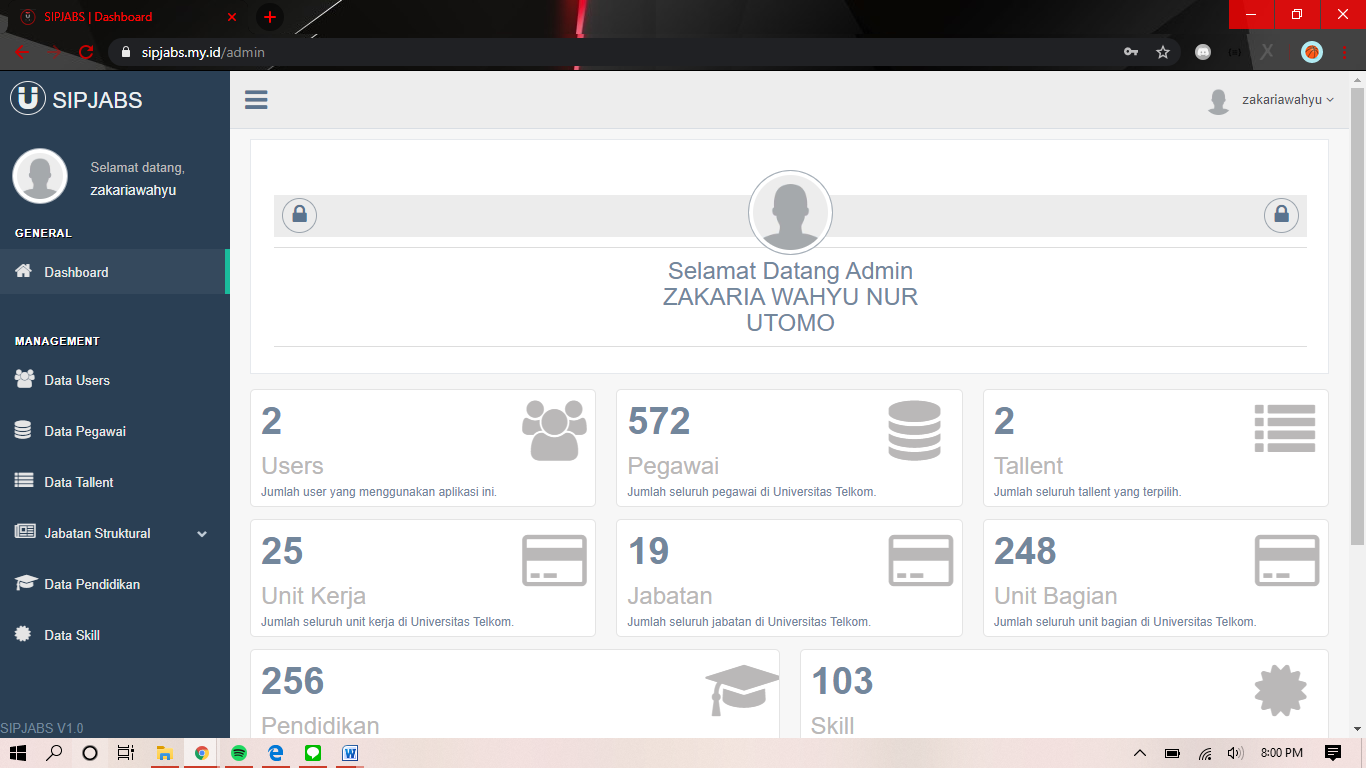
\includegraphics[width=0.8\textwidth]
		{pics/admin/implementasi/dashboard.png}
		\caption{Halaman \textit{Dashboard} Admin}
		\label{fig:CC10}
	\end{figure}
	Gambar diatas menjelaskan isi dari \textit{dashboard} admin, dibagi menjadi beberapa bagian diantaranya: terdapat jumlah \textit{user} yang dapat mengakses aplikasi SiPJabS sebagai admin maupun \textit{user}. Apabia admin menambahkan atau menghapus \textit{user} maka jumlah tersebut dapat berubah. Terdapat jumlah pegawai di Universitas Telkom. Kemudian jumlah kandidat yang sudah dipilih oleh user untuk menggantikan atau mengisi posisi yang kosong. Dibawahnya terdapat unit kerja yang didalamnya terdapat beberapa jabatan, dan didalam unit kerja juga dibagi menjadi unit bagian, agar pekerjaan lebih mudah untuk dikerjakan. Kemudian terdapat pendidikan yang dimiliki oleh pegawai Universitas Telkom, dan terakhir terdapat \textit{skill} yang dimiliki pegawai Universitas Telkom guna menunjang kerja.
	
	\newpage
	\item Halaman \textit{Profile}
	\begin{figure}
		\centering
		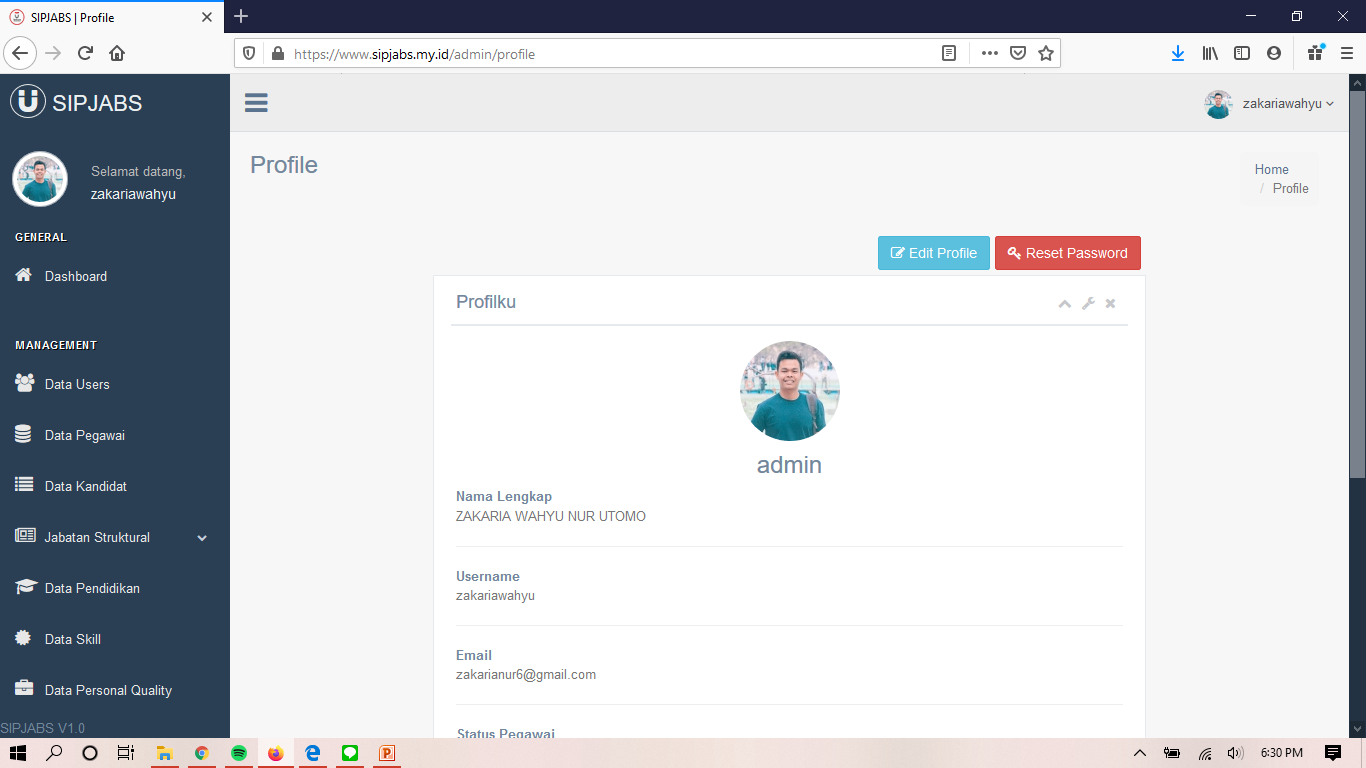
\includegraphics[width=0.8\textwidth]
		{pics/admin/implementasi/profile.png}
		\caption{Halaman \textit{Profile} Admin}
		\label{fig:CC10}
	\end{figure}
	Implementasi diatas menjelaskan bahwasannya admin dapat melihat \textit{profile} dengan mengklik \textit{username} yang berada di atas kanan, kemudian akan terdapat \textit{dropdown}, lalu klik \textit{profile}, maka akan tampil \textit{profile} dari admin.
	
	\item Halaman \textit{Edit Profile}
	\begin{figure}
		\centering
		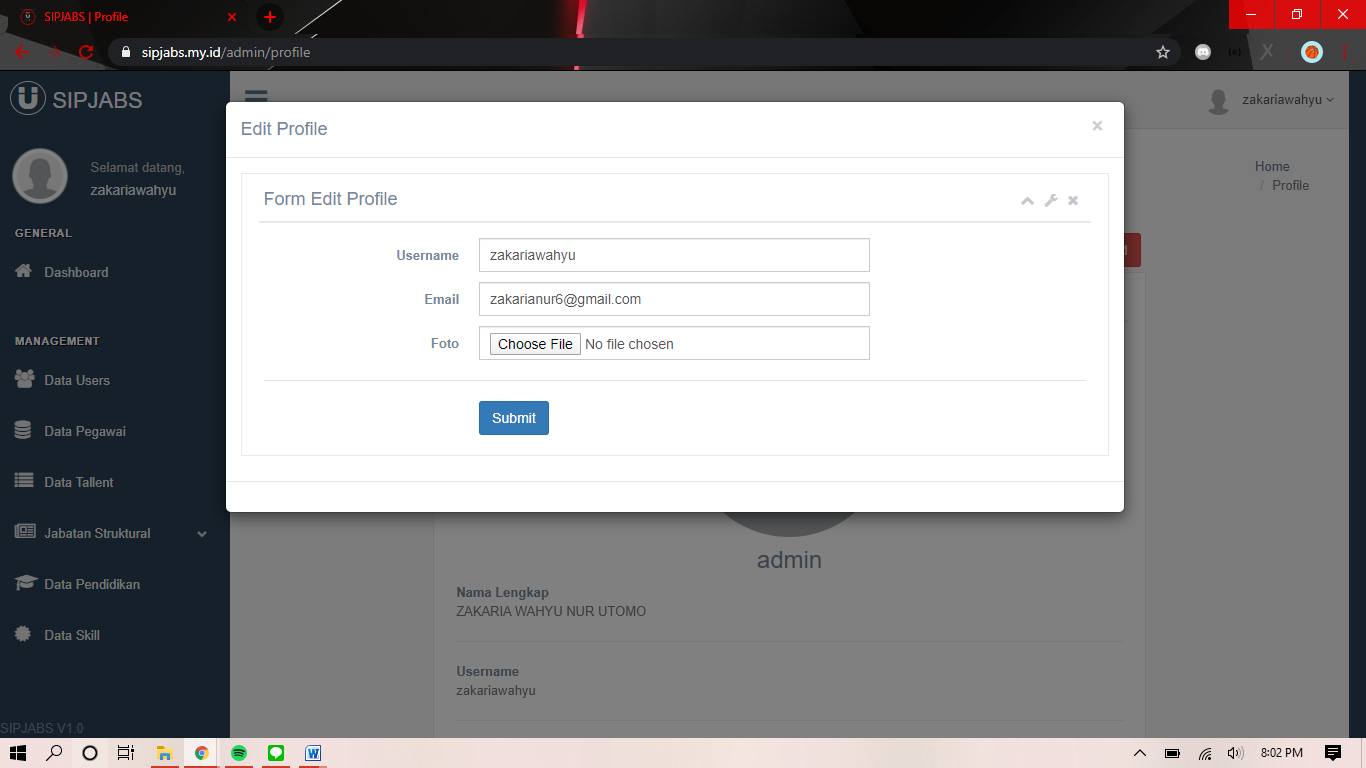
\includegraphics[width=0.8\textwidth]
		{pics/admin/implementasi/editprofile.png}
		\caption{Halaman \textit{Edit Profile} Admin}
		\label{fig:CC10}
	\end{figure}
	Gambar diatas mengimplementasikan bahwasannya admin dapat mengedit data \textit{profile} dengan mengklik \textit{button “edit profile”} kemudian dapat mengganti \textit{username} atau email dan foto. Lalu admin harus mengklik “\textit{submit}” untuk dapat menyimpan data yang sudah diperbarui. 
	
	\newpage
	\item Halaman \textit{Reset Password}
	\begin{figure}
		\centering
		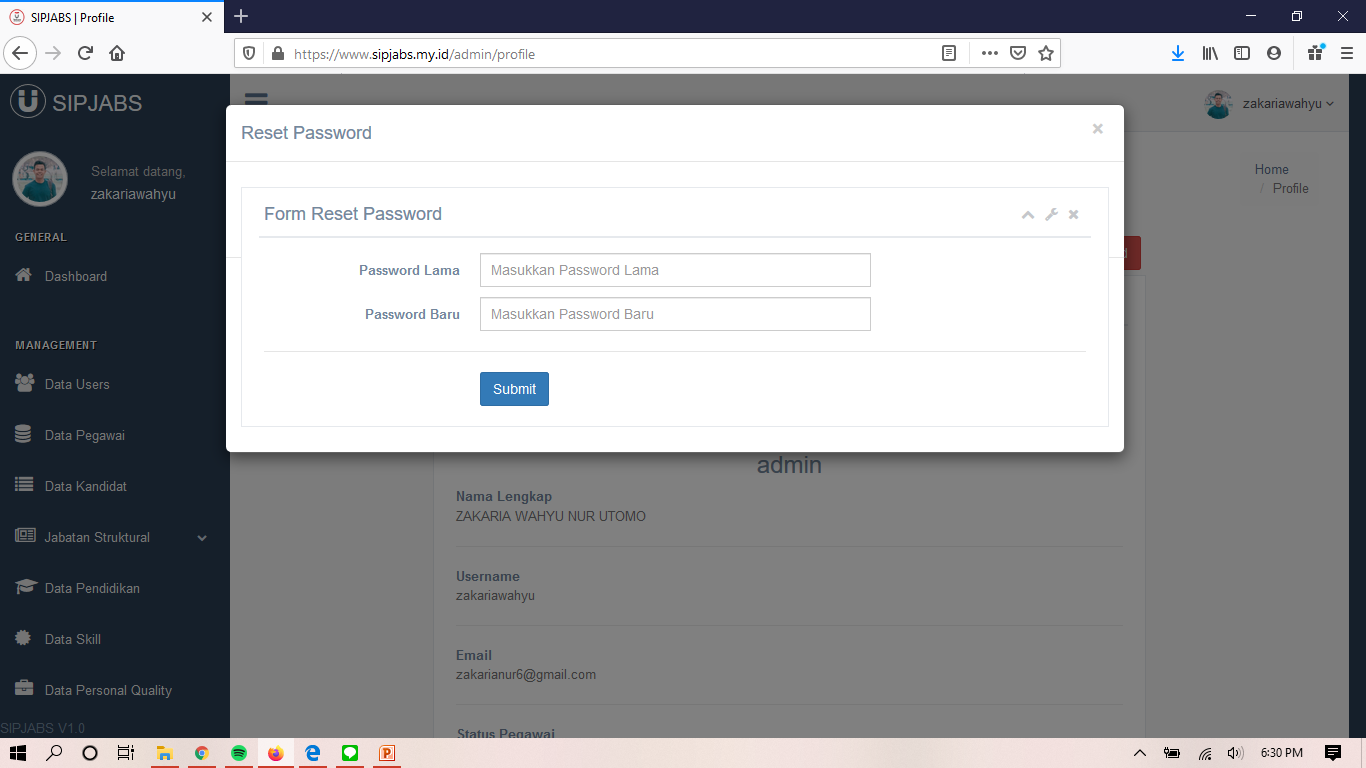
\includegraphics[width=0.8\textwidth]
		{pics/admin/implementasi/resetpassword.png}
		\caption{Halaman \textit{Reset Password} Admin}
		\label{fig:CC10}
	\end{figure}
	Implementasi diatas menandakan bahwasannya admin dapat mengganti \textit{password} apabila \textit{password} terebut sudah diketahui oleh pihak lain, dengan klik \textit{button “reset password”} kemudian akan tampil halaman \textit{pop-up} seperti diatas, admin cukup menginputkan \textit{password} lama dan \textit{password} baru, lalu klik “\textit{submit}” untuk menyimpan \textit{password} yang sudah diganti. 
	
	\item Halaman \textit{Help}
	\begin{figure}
		\centering
		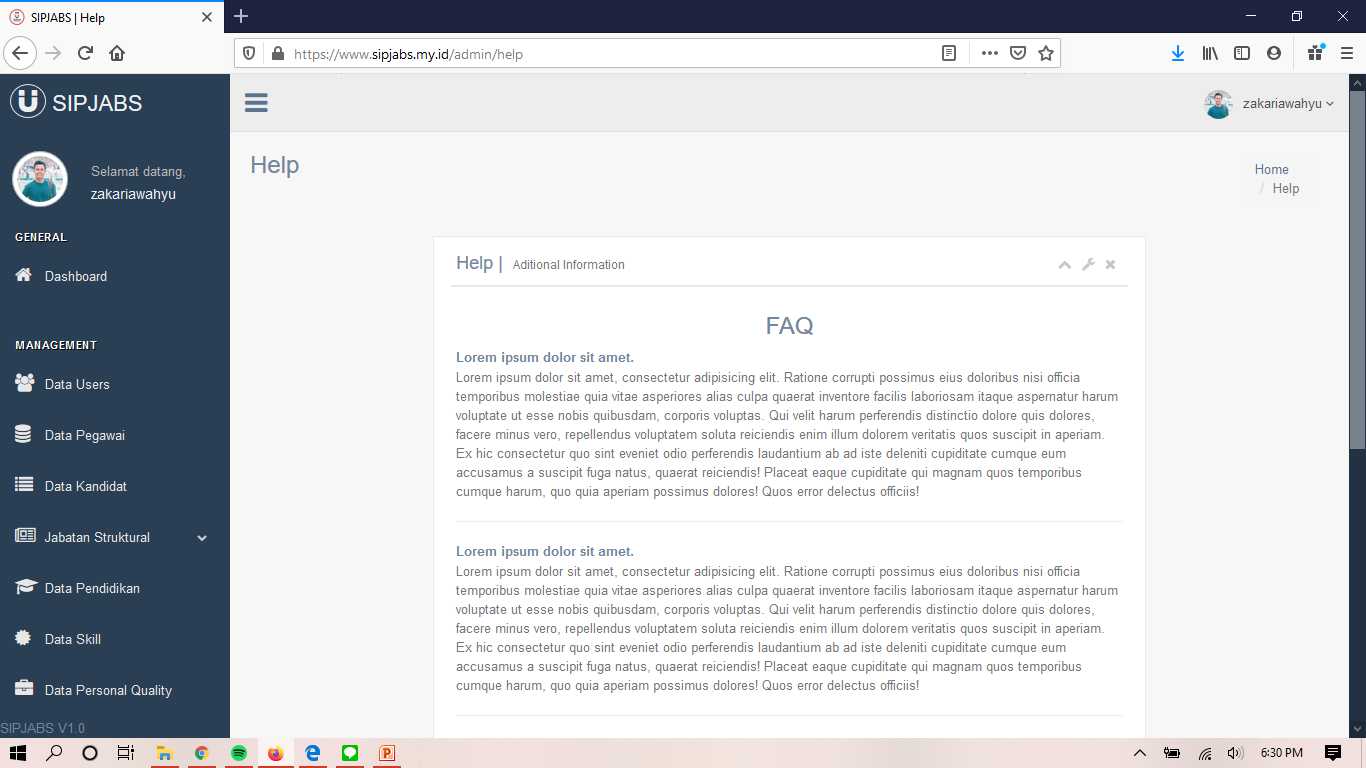
\includegraphics[width=0.8\textwidth]
		{pics/admin/implementasi/help.png}
		\caption{Halaman \textit{Help} Admin}
		\label{fig:CC10}
	\end{figure}

	\newpage
	\item Halaman Data \textit{Users}
	\begin{figure}
		\centering
		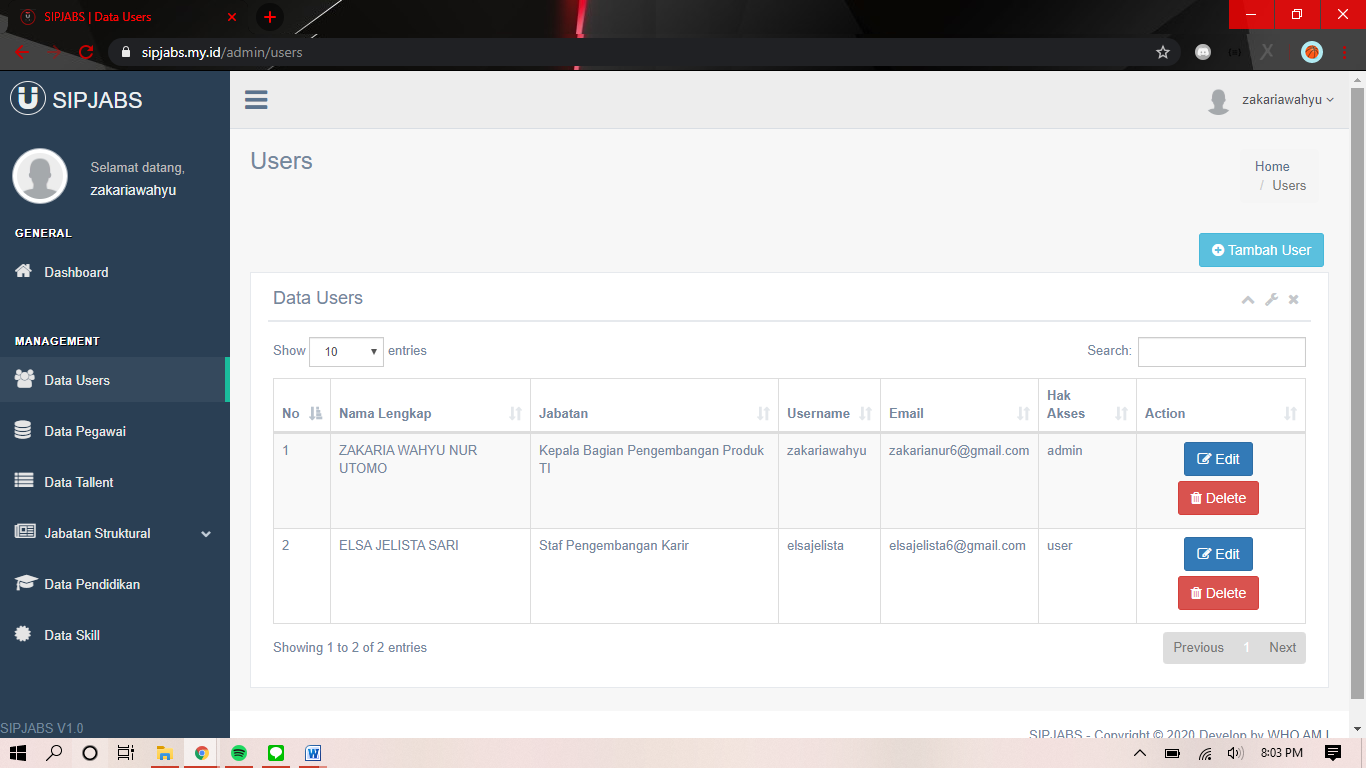
\includegraphics[width=0.8\textwidth]
		{pics/admin/implementasi/datausers.png}
		\caption{Halaman Data \textit{Users} - Admin}
		\label{fig:CC10}
	\end{figure}
	Gambar diatas menjelaskan isi dari halaman data \textit{users}, dimana admin dapat mengelola \textit{users} yang bisa mengakses aplikasi \textbf{SiPJabS}, karena apikasi ini hanya dapat diakses oleh orang-orang tententu. 
	
	\item Halaman \textit{Edit} Data \textit{Users}
	\begin{figure}
		\centering
		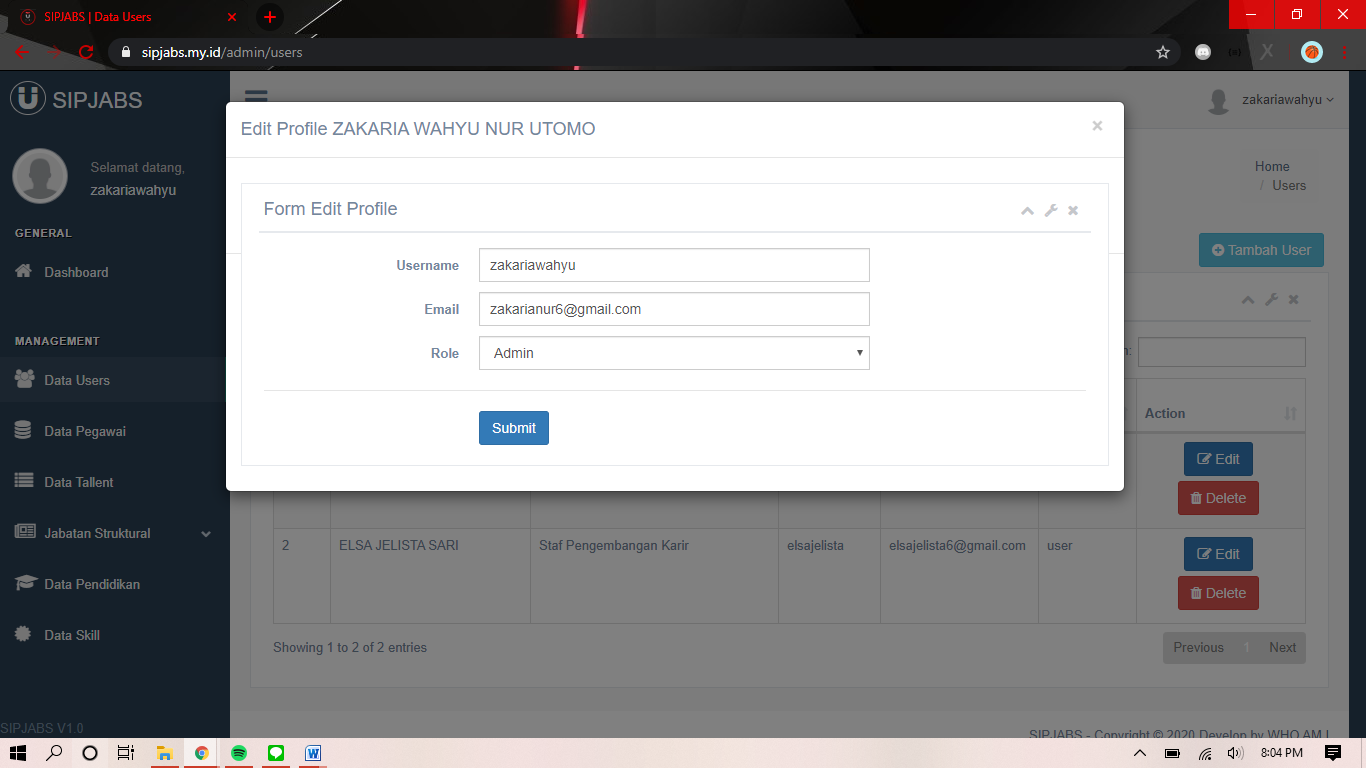
\includegraphics[width=0.8\textwidth]
		{pics/admin/implementasi/editusers.png}
		\caption{Halaman \textit{Edit} Data \textit{Users} - Admin}
		\label{fig:CC10}
	\end{figure}
	Gambar diatas menjelaskan bahwasannya data \textit{users} dapat diedit seperti \textit{username}, email, dan \textit{role} yang digunakan sebagai admin atau \textit{user}. Apabila data sudah diubah admin dapat mengklik \textit{button “Submit”} untuk menyelesaikan proses.
	
	\newpage
	\item Halaman Tambah \textit{Users}
	\begin{figure}
		\centering
		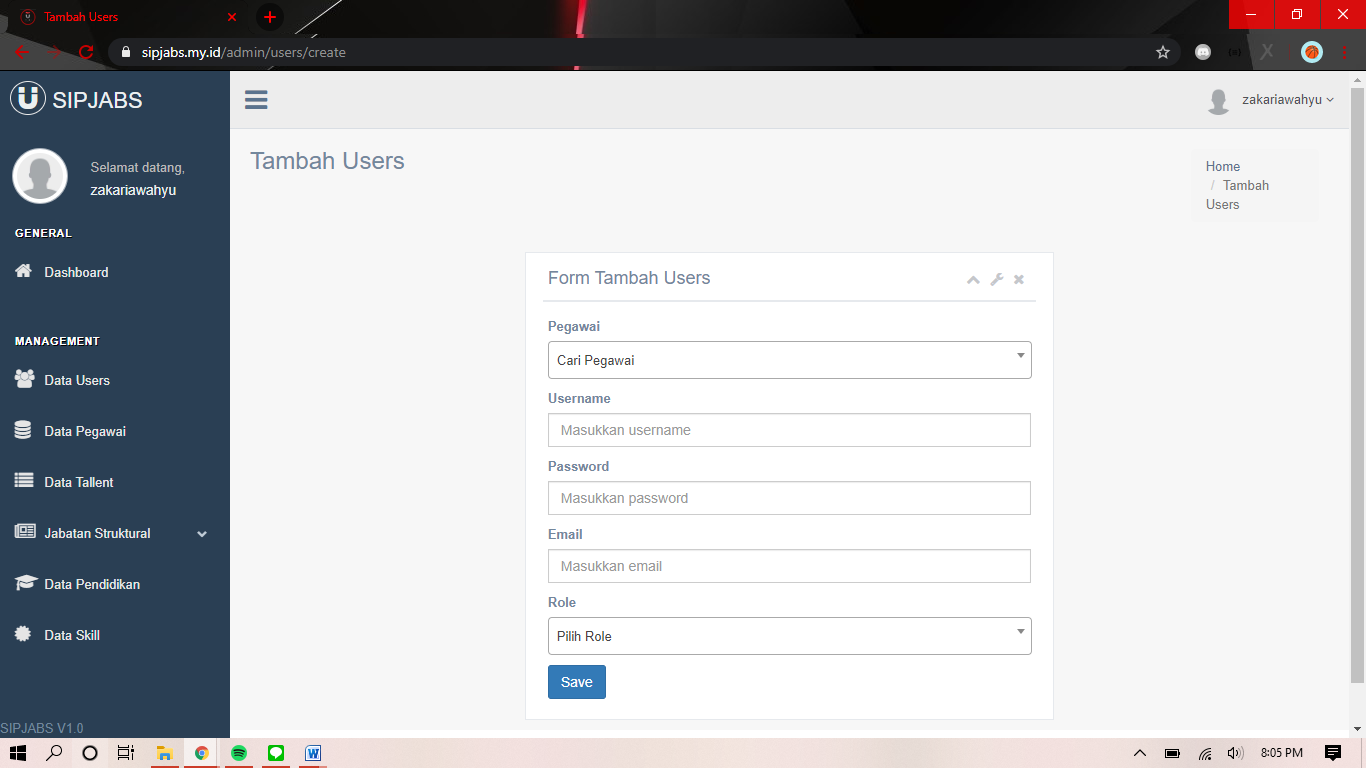
\includegraphics[width=0.8\textwidth]
		{pics/admin/implementasi/tambahusers.png}
		\caption{Halaman Tambah \textit{Users} - Admin}
		\label{fig:CC10}
	\end{figure}
	Dari tampilan diatas dapat dijelaskan, hanya admin saja yang dapat menambahkan data \textit{user}, namun harus sesuai dengan perintah dan \textit{job description} pegawai. Dengan mencari nama pegawai, menginputkan \textit{username}, \textit{password}, email, dan \textit{role}nya sebagai admin atau \textit{user}. Untuk mengakhiri proses admin dapat menyimpan apabila sudah disimpan akan terdapat \textit{pop-up}.
	
	\item Halaman Data Pegawai
	\begin{figure}
		\centering
		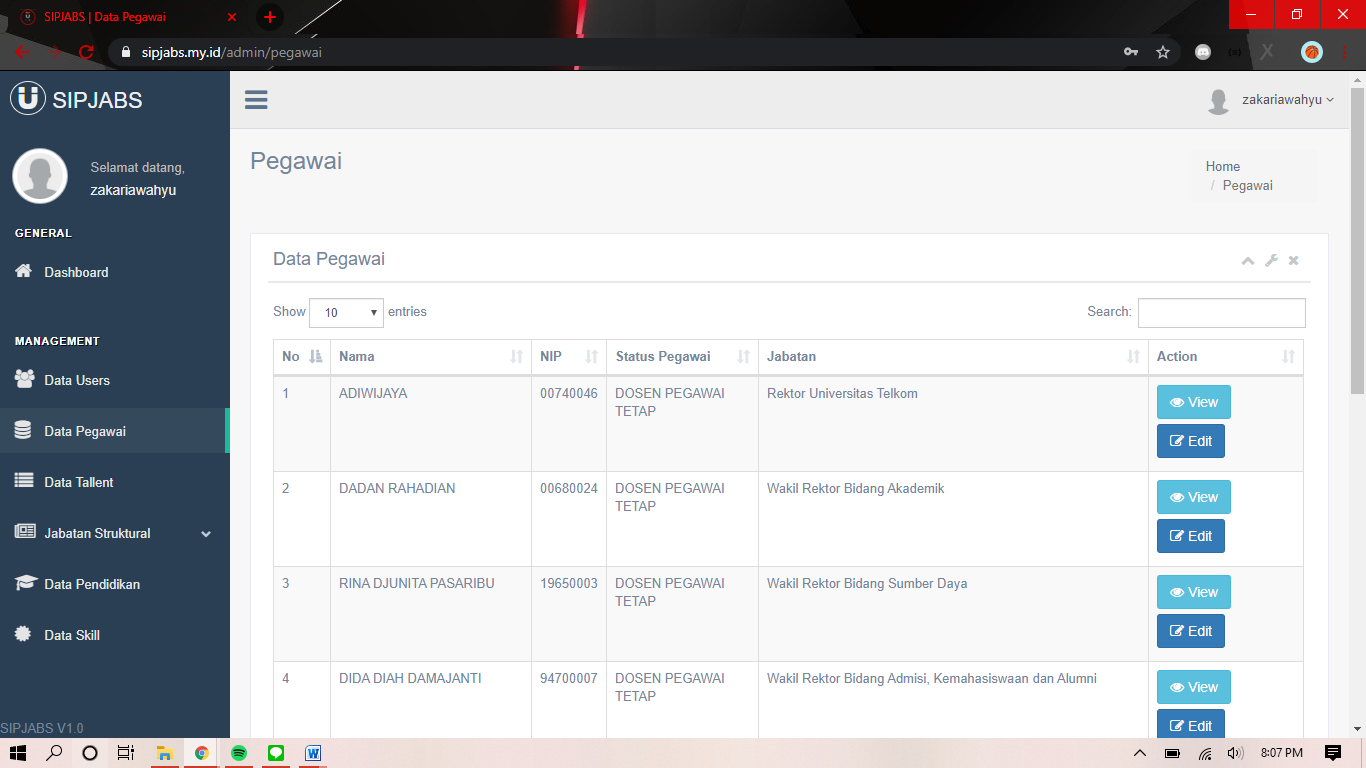
\includegraphics[width=0.8\textwidth]
		{pics/admin/implementasi/datapegawai.png}
		\caption{Halaman Data Pegawai - Admin}
		\label{fig:CC10}
	\end{figure}
	Dari tampilan diatas dijelaskan bahwasannya admin dapat melihat data seluruh pegawai yang ada di Universitas Telkom dengan mengklik menu “Data Pegawai” yang ada di sebelah kiri.
	
	\item Halaman \textit{View Detail} Pegawai
	\begin{figure}
		\centering
		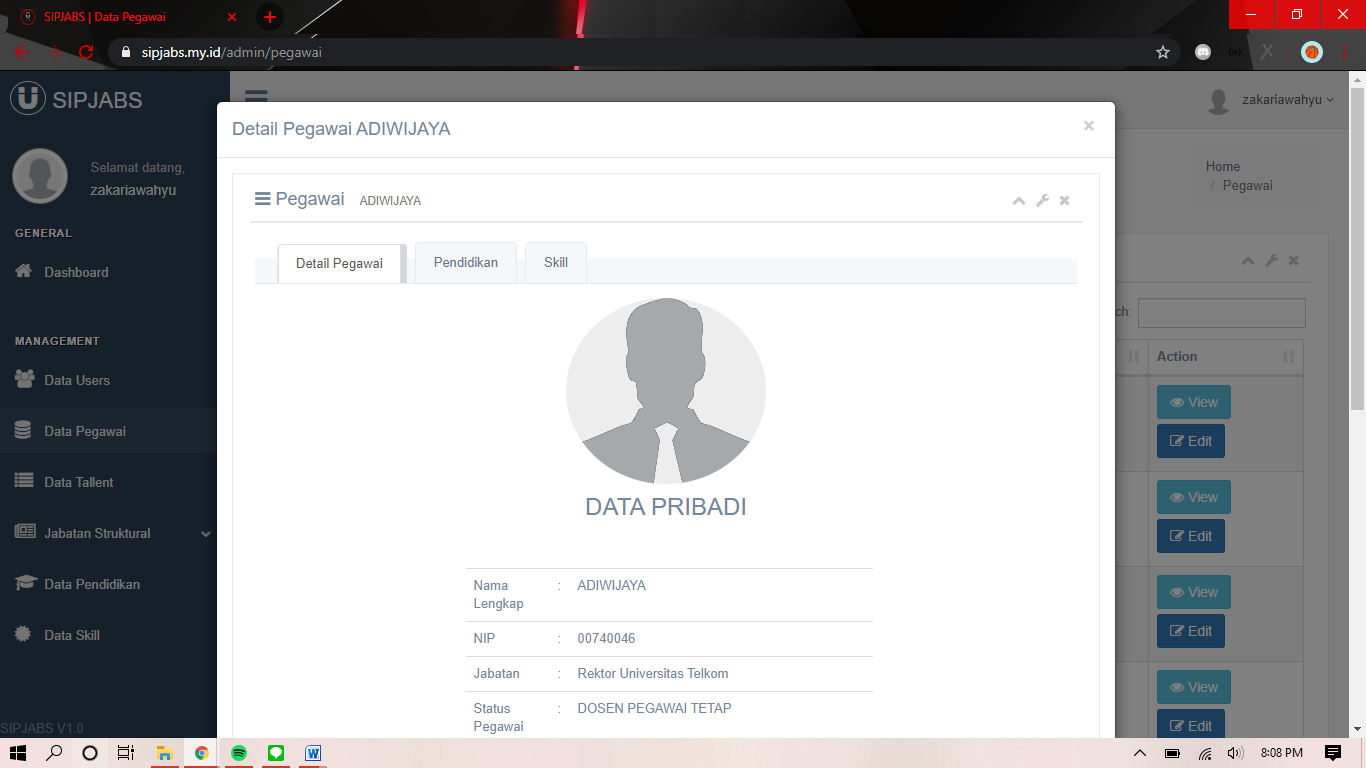
\includegraphics[width=0.8\textwidth]
		{pics/admin/implementasi/viewdetailpegawai.png}
		\caption{Halaman \textit{View Detail} Pegawai - Admin}
		\label{fig:CC10}
	\end{figure}
	Untuk implementasi \textit{view detail} pegawai admin dapat mengklik \textit{button view}, maka akan tampil seperti gambar diatas. Terdapat data pribadi dari pegawai yang dapat dilihat diantaranya: nama lengkap, NIP, jabatan, status pegawai, masa kerja, tempat lahir, tanggal lahir, status perkawinan, golongan darah, jenis kelamin, agama, tinggi badan, berat badan, dan alamat.
	
	\item Halaman \textit{Edit} Pegawai
	\begin{figure}
		\centering
		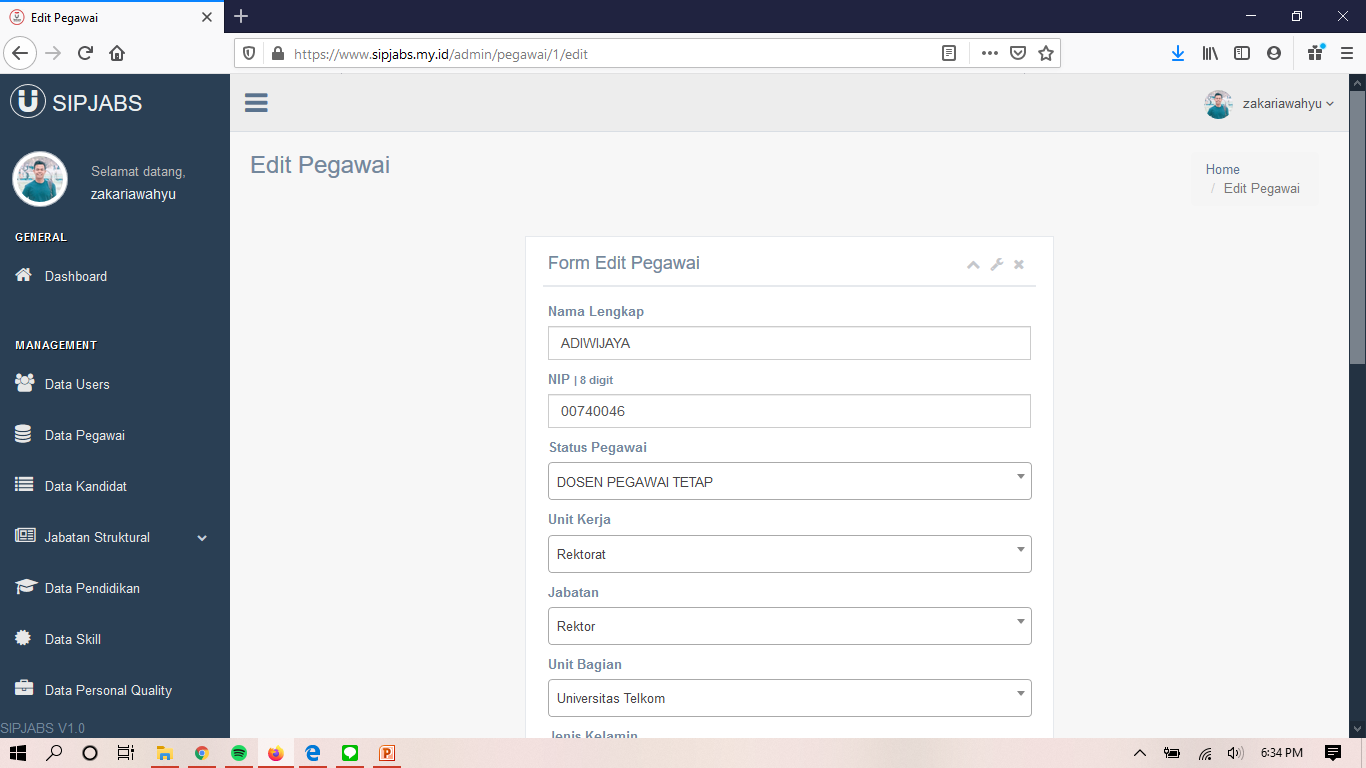
\includegraphics[width=0.8\textwidth]
		{pics/admin/implementasi/editpegawai.png}
		\caption{Halaman \textit{Edit} Pegawai - Admin}
		\label{fig:CC10}
	\end{figure}
	Untuk implementasi \textit{edit} pegawai admin dapat mengklik \textit{button} edit, maka akan tampil seperti gambar diatas dan dapat mengedit data yang ada.
	
	\newpage
		\item Halaman Data Kandidat
	\begin{figure}
		\centering
		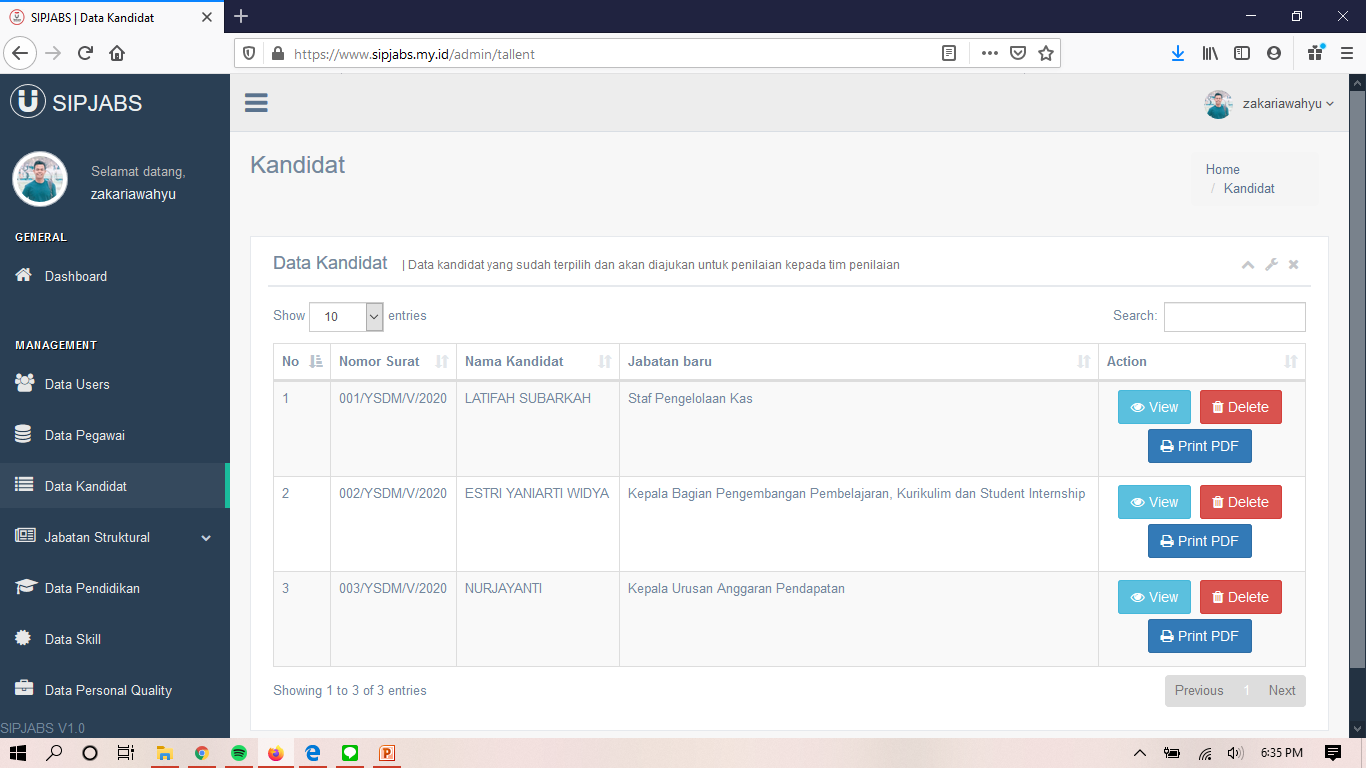
\includegraphics[width=0.8\textwidth]
		{pics/admin/implementasi/datatallent.png}
		\caption{Halaman Data Kandidat - Admin}
		\label{fig:CC10}
	\end{figure}
	Gambar diatas menampilkan halaman data kandidat yang dapat dilihat apabila admin mengklik menu “Data Kandidat”. Terdapat data kandidat yang sudah dipilih oleh \textit{user}, sesuai dengan \textit{requirement} yang telah ditetapkan perusahaan guna mengganti atau mengisi posisi yang kosong.  
	
	\item Halaman \textit{View Detail} Kandidat
	\begin{figure}
		\centering
		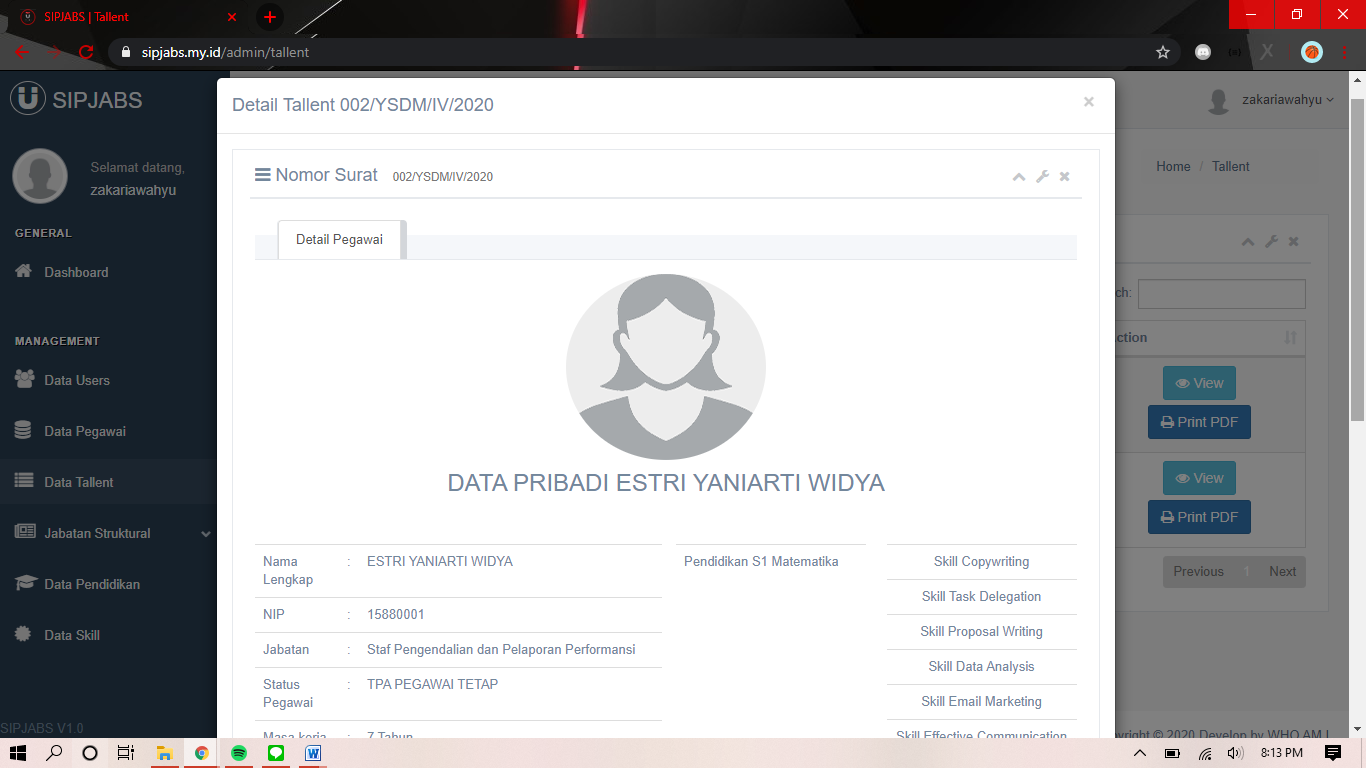
\includegraphics[width=0.8\textwidth]
		{pics/admin/implementasi/viewdetailtallent.png}
		\caption{Halaman \textit{View Detail} Kandidat - Admin}
		\label{fig:CC10}
	\end{figure}
	Tampilan diatas akan muncul apabila admin mengklik \textit{button “view”}. Kemudian tampil \textit{detail} data pegawai yang suda dipilih oleh \textit{user}, seperti data pribadi, jenjang pendidikan, dan \textit{skill}. 
	
	\newpage
	\item Halaman Data Unit Kerja
	\begin{figure}
		\centering
		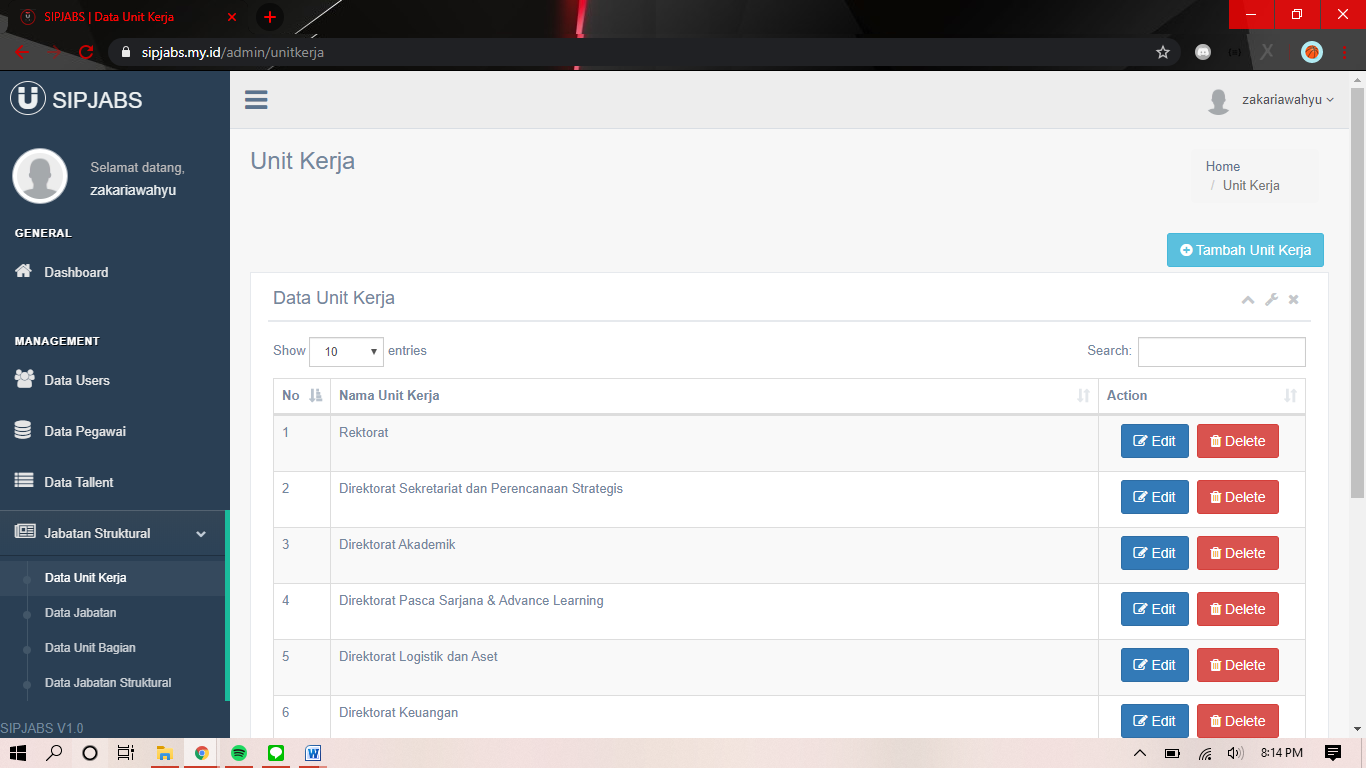
\includegraphics[width=0.8\textwidth]
		{pics/admin/implementasi/dataunitkerja.png}
		\caption{Halaman Data Unit Kerja - Admin}
		\label{fig:CC10}
	\end{figure}
	Untuk implementasi diatas admin harus klik “jabatan struktural” kemudian akan terdapat \textit{dropdown}, lalu klik “data unit kerja” maka akan menampilkan data unit kerja yang berada di Universitas Telkom dari rektorat hingga ke fakultas. 
	
	\item Halaman \textit{Edit} Unit Kerja
	\begin{figure}
		\centering
		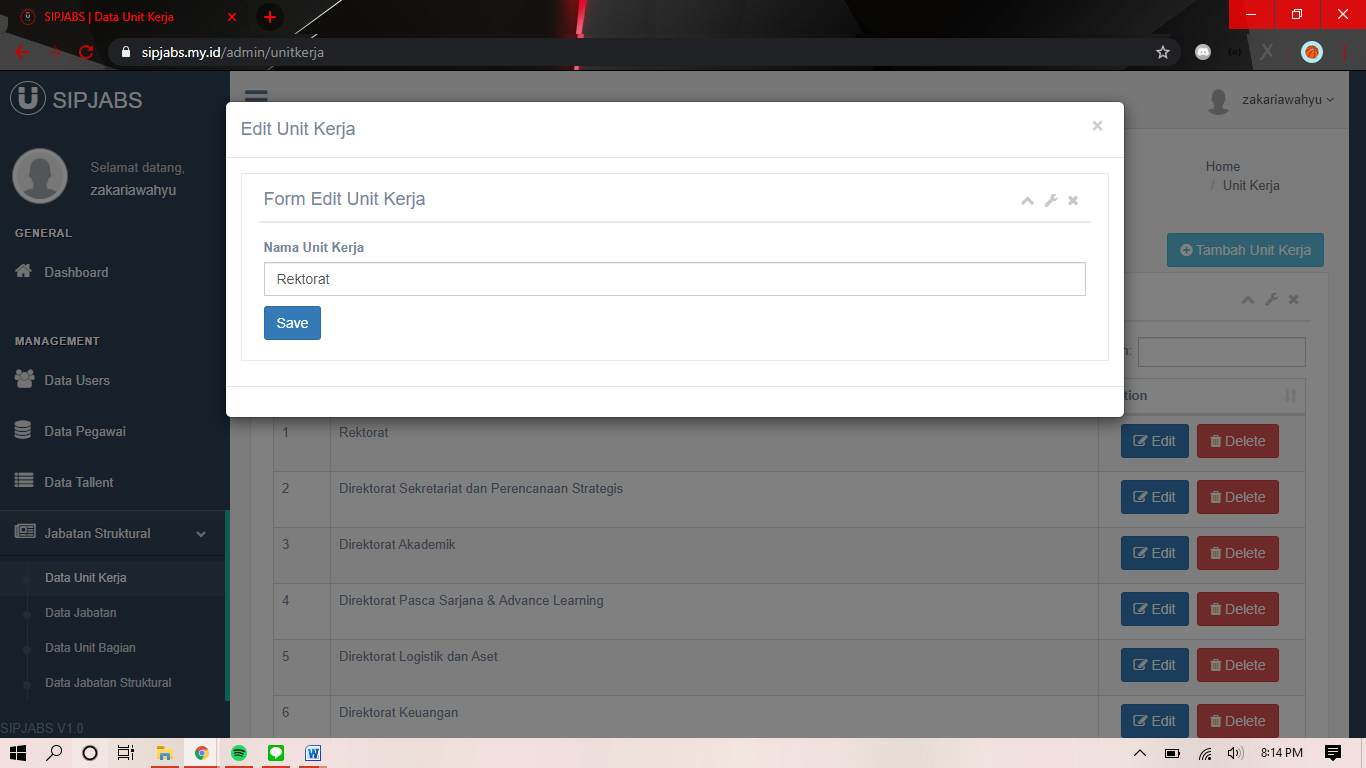
\includegraphics[width=0.8\textwidth]
		{pics/admin/implementasi/editunitkerja.png}
		\caption{Halaman \textit{Edit} Unit Kerja - Admin}
		\label{fig:CC10}
	\end{figure}
	Gambar diatas akan muncul apabila admin mengklik \textit{button “edit”} kemudian akan tampil \textit{pop-up} edit unit kerja, apabila nama unit kerja mengalami perubahan yang sudah ditetapkan. 
	
	\newpage
	\item Halaman Tambah Unit Kerja
	\begin{figure}
		\centering
		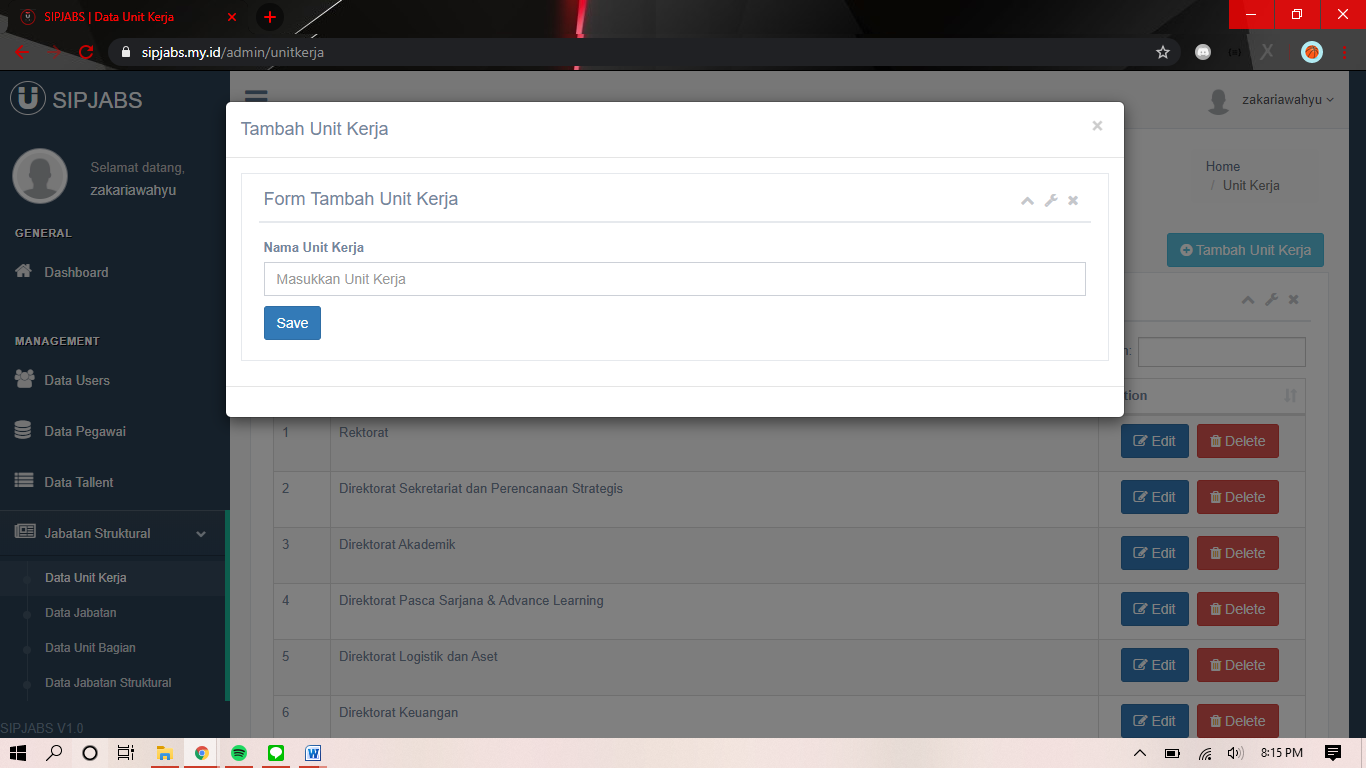
\includegraphics[width=0.8\textwidth]
		{pics/admin/implementasi/tambahunitkerja.png}
		\caption{Halaman Tambah Unit Kerja - Admin}
		\label{fig:CC10}
	\end{figure}
	Implementasi diatas akan muncul apabila admin mengklik \textit{button} “tambah unit kerja”, apabila terdapat unit kerja baru yang sudah ditetapkan, maka admin dapat menambahkannya. Untuk menyelesaikan proses admin harus mengklik \textit{button “save”}, kemudian data akan tersimpan.
	
	\item Halaman Data Jabatan
	\begin{figure}
		\centering
		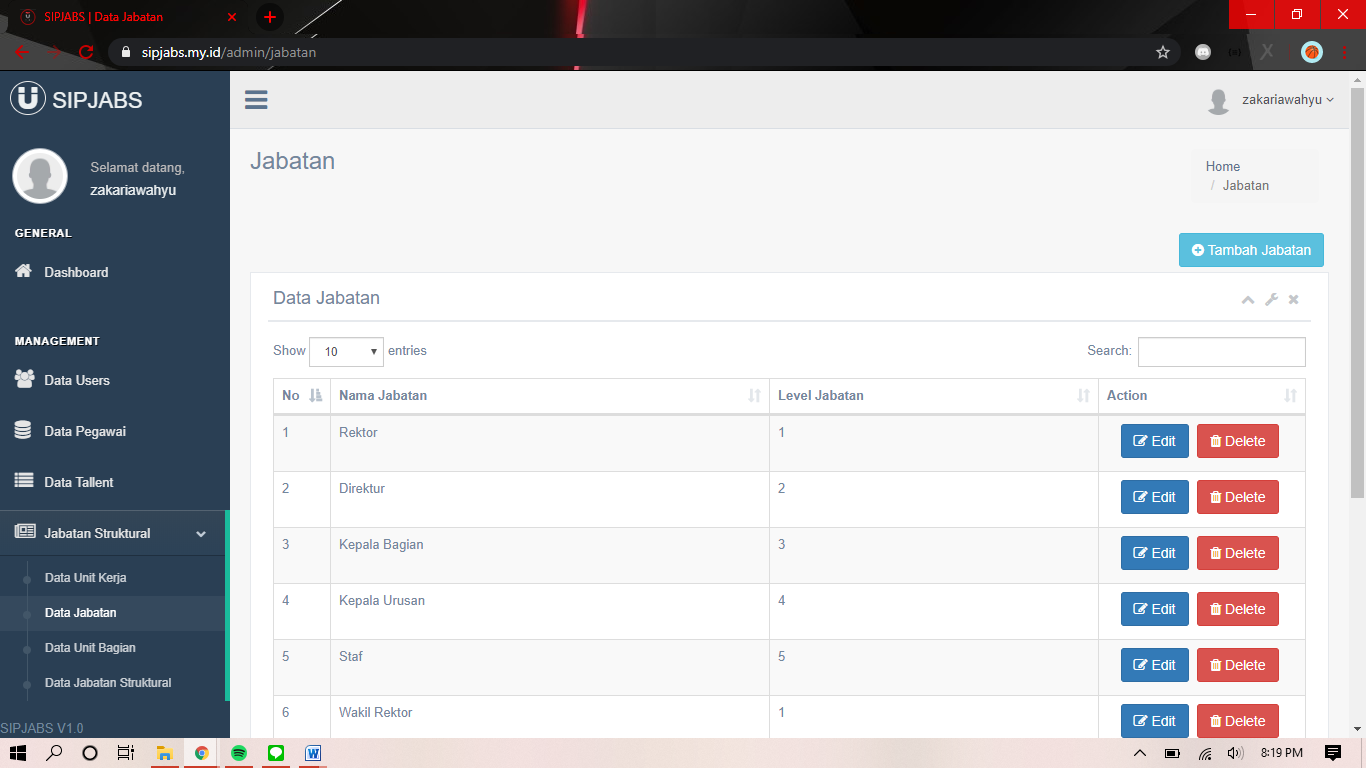
\includegraphics[width=0.8\textwidth]
		{pics/admin/implementasi/datajabatan.png}
		\caption{Halaman Data Jabatan - Admin}
		\label{fig:CC10}
	\end{figure}
	Gambar diatas menampilkan data jabatan apabila admin mengklik menu “data jabatan” pada \textit{dropdown} ”jabatan struktural”. Terdapat nama-nama jabatan yang ada di Universitas Telkom yang akan terhubung dengan unit kerja dan unit bagian.  
	
	\item Halaman \textit{Edit} Jabatan
	\begin{figure}
		\centering
		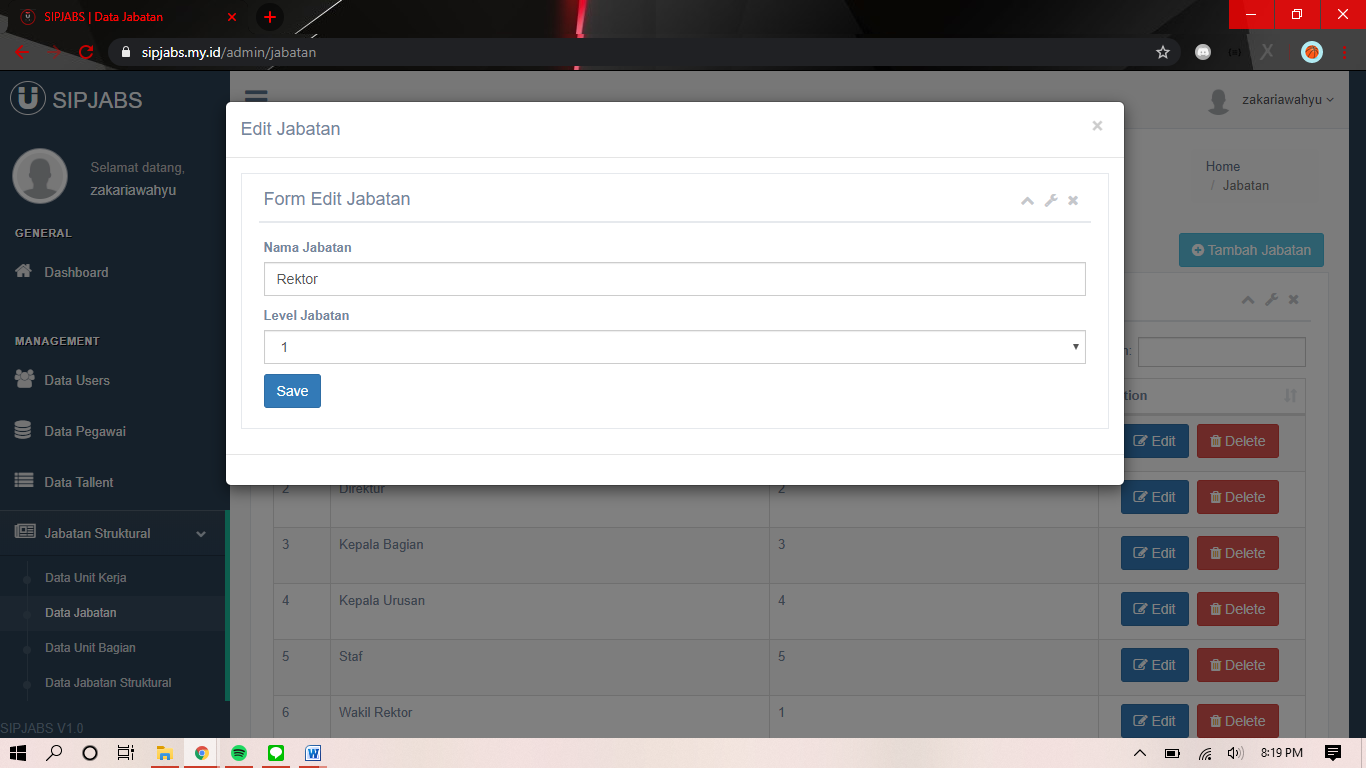
\includegraphics[width=0.8\textwidth]
		{pics/admin/implementasi/editjabatan.png}
		\caption{Halaman \textit{Edit} Jabatan - Admin}
		\label{fig:CC10}
	\end{figure}
	Untuk tampilan diatas adalah \textit{form edit} jabatan, admin dapat mengklik \textit{button “edit”} kemudian menginputkan nama jabatan serta level jabatan, dan menyimpannya untuk mengakhiri proses, kemudian data akan tersimpan.
	
	\item Halaman Tambah Jabatan
	\begin{figure}
		\centering
		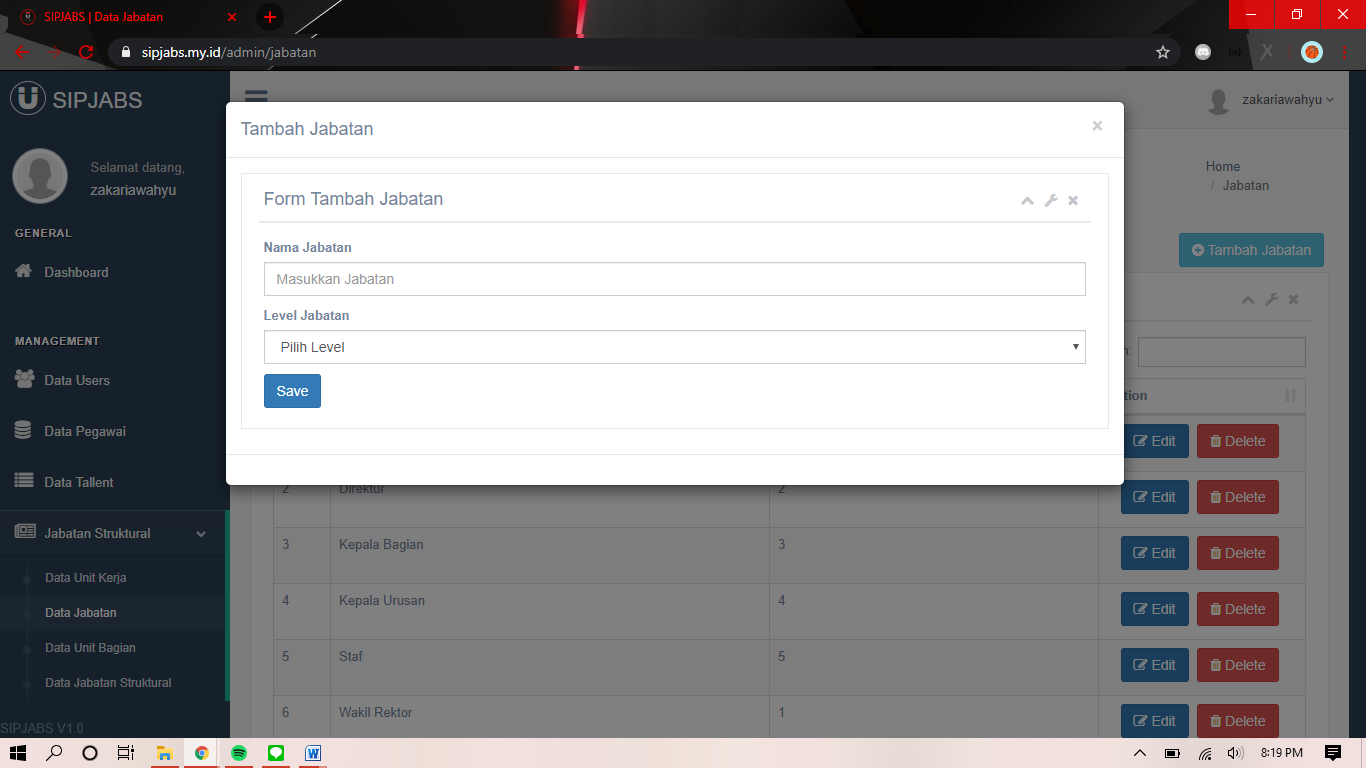
\includegraphics[width=0.8\textwidth]
		{pics/admin/implementasi/tambahjabatan.png}
		\caption{Halaman Tambah Jabatan - Admin}
		\label{fig:CC10}
	\end{figure}
	Gambar diatas menampilkan \textit{pop-up form} tambah jabatan, tampilan tersebut akan muncul apabila admin mengklik \textit{button} “tambah jabatan”. Kemudian admin menginputkan nama jabatan dan level jabatan untuk membuat jabatan baru yang sudah ditetapkan. Lalu simpan data tersebut dengan mengklik \textit{button “save”} maka data akan tesimpan di jabatan.
	
	\item Halaman Data Unit Bagian
	\begin{figure}
		\centering
		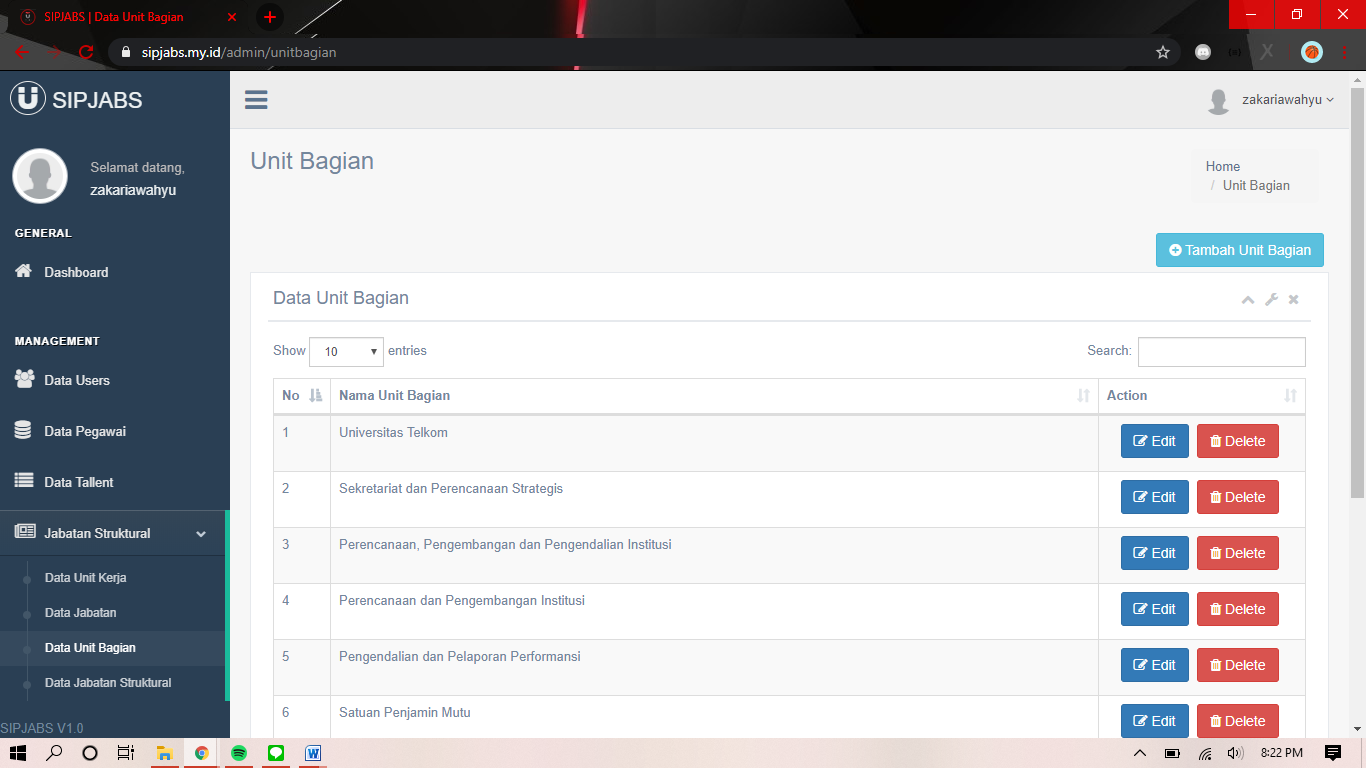
\includegraphics[width=0.8\textwidth]
		{pics/admin/implementasi/dataunitbagian.png}
		\caption{Halaman Data Unit Bagian - Admin}
		\label{fig:CC10}
	\end{figure}
	Untuk tampilan diatas adalah tampilan dari data unit bagian, didapat apabila admin mengklik \textit{dropdown} “jabatan struktural” pada menu kemudian mengklik “data unit bagian”, halaman ini menjelaskan bagian dari unit kerja yang ada di Universitas Telkom. Diharapkan dapat menyelesaikan pekerjaan sesuai dengan unit bagian masing-masing secara efektif dan maksimal.
	
	\item Halaman \textit{Edit} Unit Bagian
	\begin{figure}
		\centering
		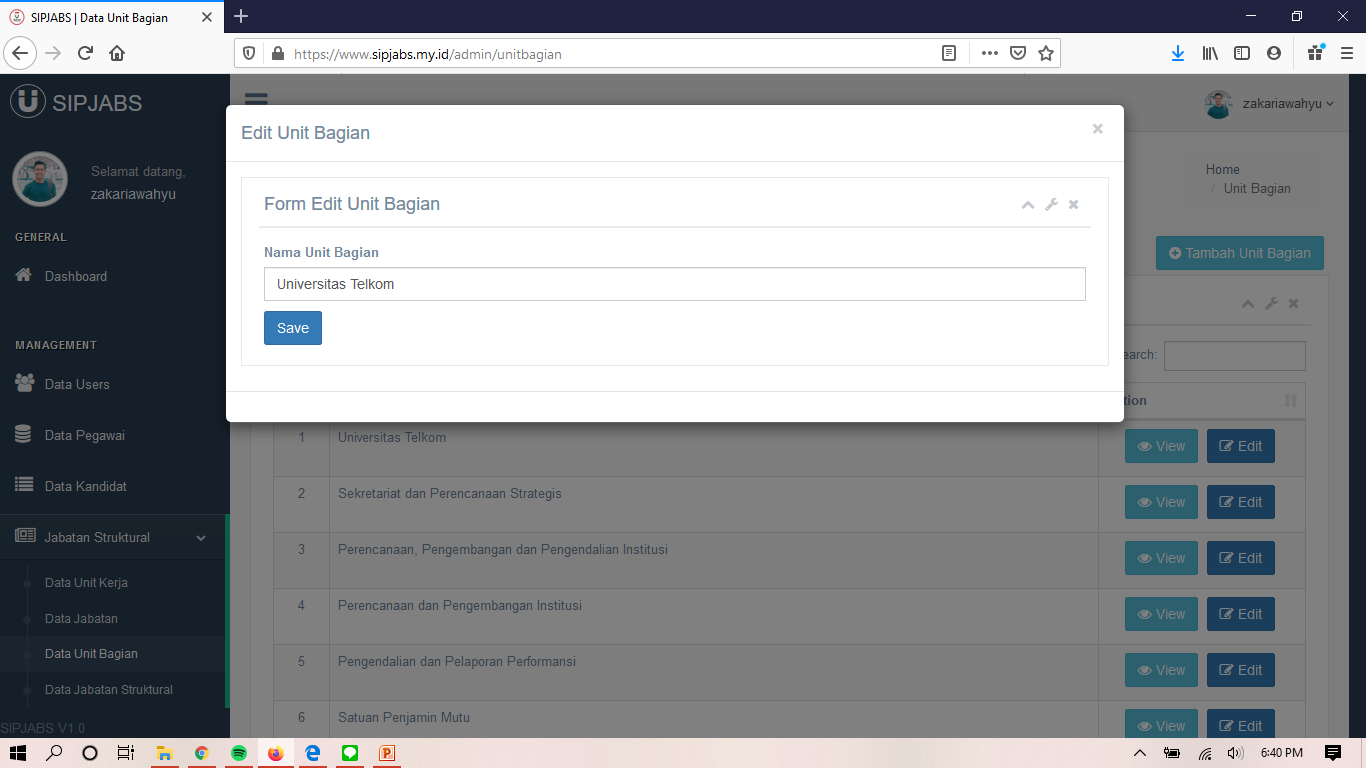
\includegraphics[width=0.8\textwidth]
		{pics/admin/implementasi/editunitbagian.png}
		\caption{Halaman \textit{Edit} Unit Bagian - Admin}
		\label{fig:CC10}
	\end{figure}
	Gambar diatas menampilkan \textit{form edit} unit bagian, didapat apabila admin mengklik \textit{button ”edit”} kemudian admin dapat menginputkan nama unit bagian yang baru dan sesuai dengan ketetapan, terakhir klik \textit{button “save”} sehingga data akan tersimpan kembali.
	
	\item Halaman Tambah Unit Bagian
	\begin{figure}
		\centering
		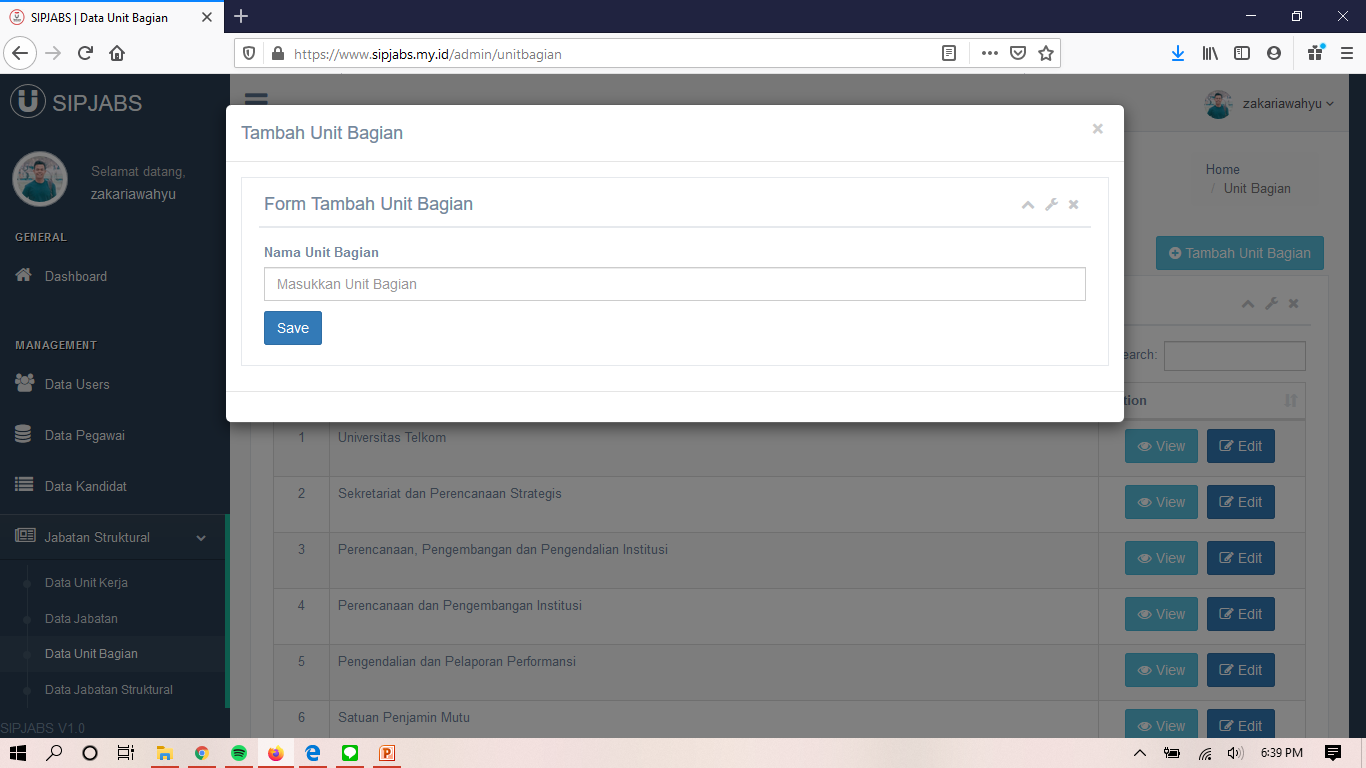
\includegraphics[width=0.8\textwidth]
		{pics/admin/implementasi/tambahunitbagian.png}
		\caption{Halaman Tambah Unit Bagian - Admin}
		\label{fig:CC10}
	\end{figure}
	Implementasi diatas menunjukkan bahwasannya admin dapat menambah data unit bagian dengan cara klik \textit{button} “tambah unit bagian” dan menginputkan nama unit bagian dan menyimpannya dengan mengklik \textit{button “save”}, kemudian data akan tersimpan didalam data unit bagian. 
	
	\item Halaman Data Jabatan Struktural
	\begin{figure}
		\centering
		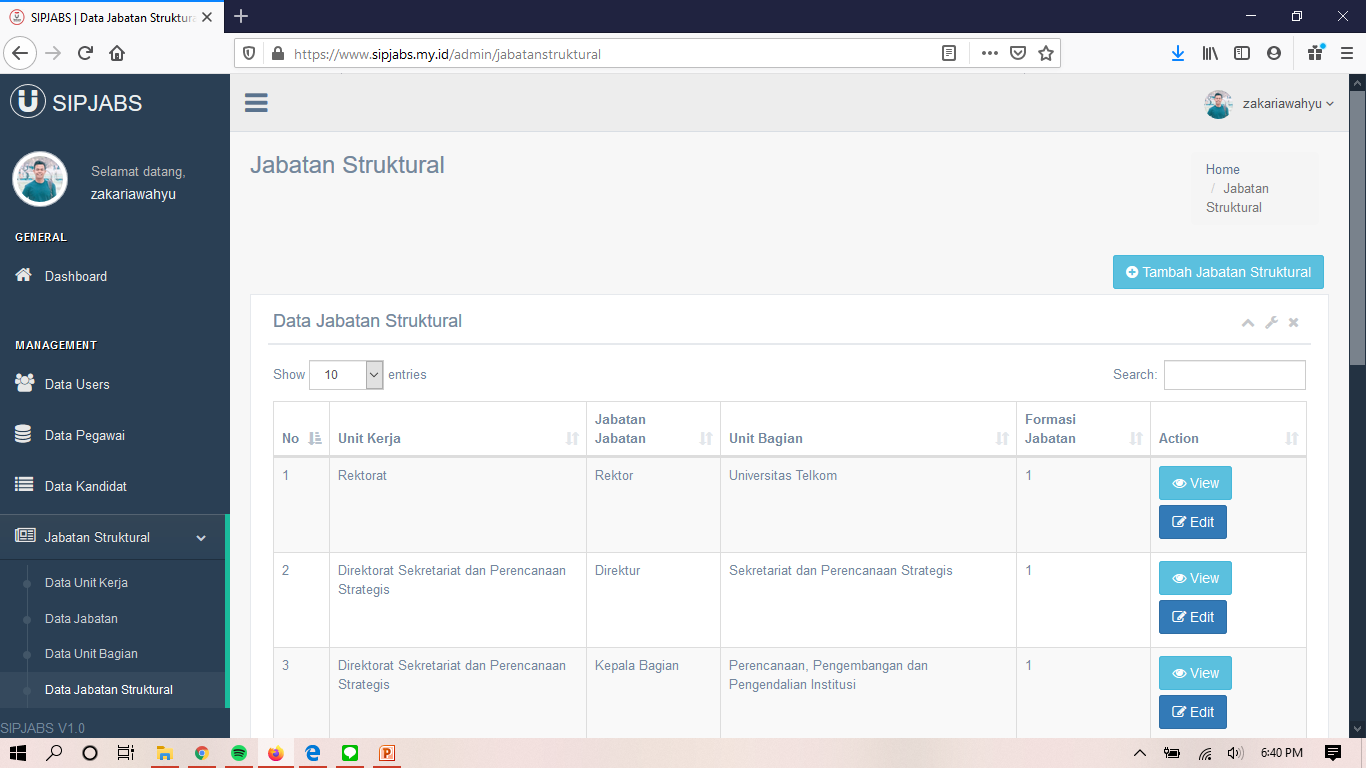
\includegraphics[width=0.8\textwidth]
		{pics/admin/implementasi/datajabstruk.png}
		\caption{Halaman Data Jabatan Struktural - Admin}
		\label{fig:CC10}
	\end{figure}
	Untuk implementasi dari tampilan diatas admin dapat mengklik \textit{dropdown} “jabatan struktural” kemudian mengklik menu “data jabatan struktural”, makan akan tampil halaman jabatan struktural yang ada di Universitas Telkom. Terdiri dari unit kerja, jabatan, unit bagian serta formasi jabatan. 
	
	\item Halaman \textit{Edit} Jabatan Struktural
	\begin{figure}
		\centering
		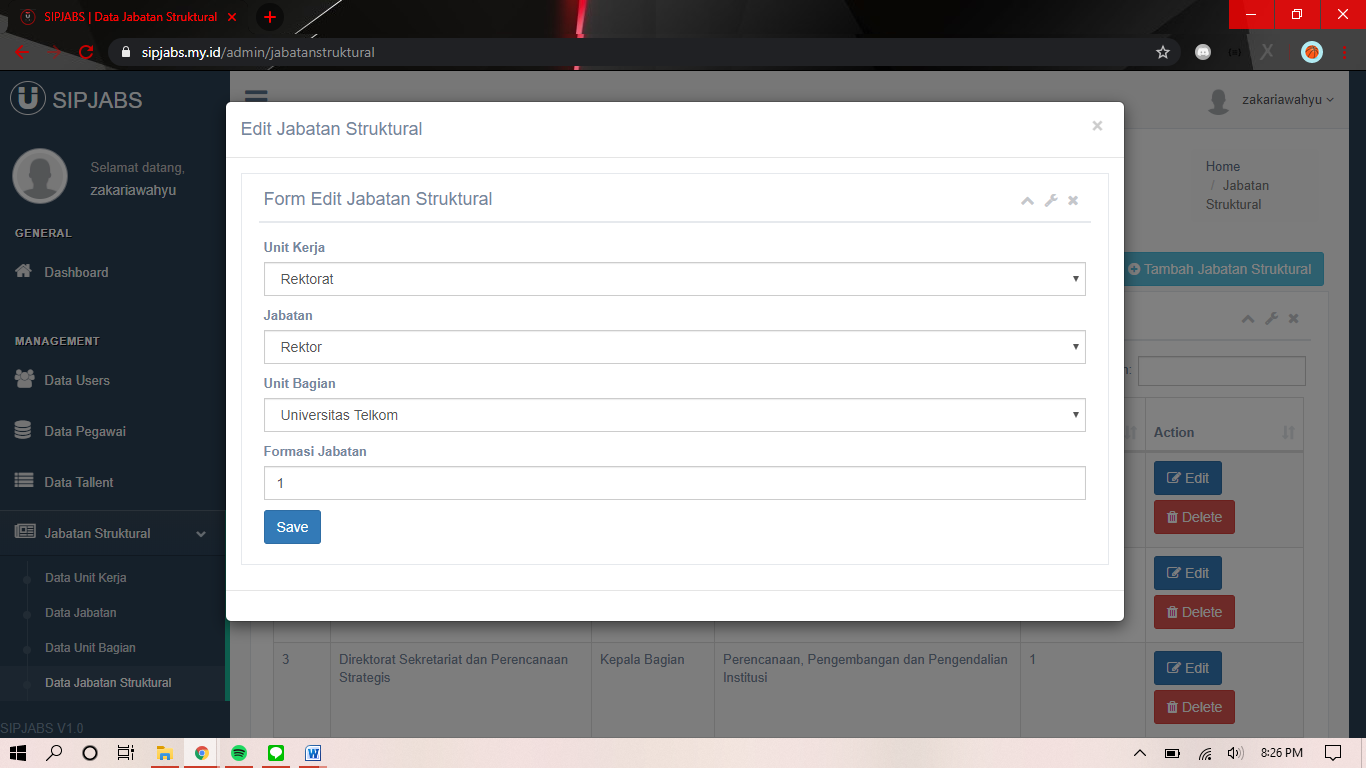
\includegraphics[width=0.8\textwidth]
		{pics/admin/implementasi/editjabstruk.png}
		\caption{Halaman \textit{Edit} Jabatan Struktural - Admin}
		\label{fig:CC10}
	\end{figure}
	Gambar diatas mengimplementasikan \textit{pop-up} dari \textit{form edit} jabatan struktural, dimana admin harus menginputkan unit kerja, jabatan, unit bagian, dan formasi jabatan, lalu untuk mengakhiri proses admin harus mengklik \textit{button “save”} kemudian data yang diedit akan tersimpan. 
	
	\item Halaman Tambah Jabatan Struktural
	\begin{figure}
		\centering
		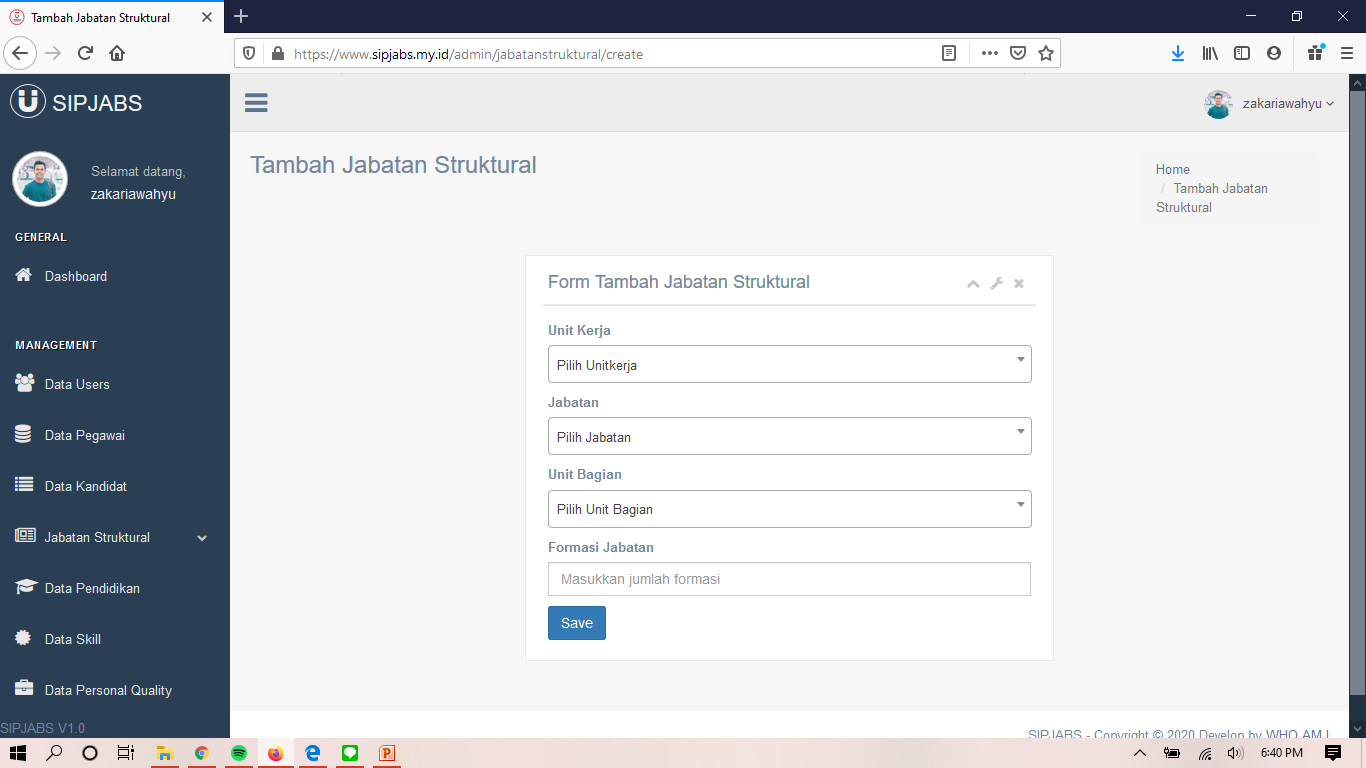
\includegraphics[width=0.8\textwidth]
		{pics/admin/implementasi/tambahjabstruk.png}
		\caption{Halaman Tambah Jabatan Struktural - Admin}
		\label{fig:CC10}
	\end{figure}
	Untuk tampilan diatas adalah \textit{form} tambah jabatan stuktural, didapat apabila admin mengklik \textit{button} “tambah jabatan struktural”, kemudian admin harus menginputkan data seperti unit kerja, jabatan, unit bagian, dan formasi jabatan, kemudian klik \textit{button “save”} untuk mengakhiri proses.
	
	\item Halaman Data Pendidikan
	\begin{figure}
		\centering
		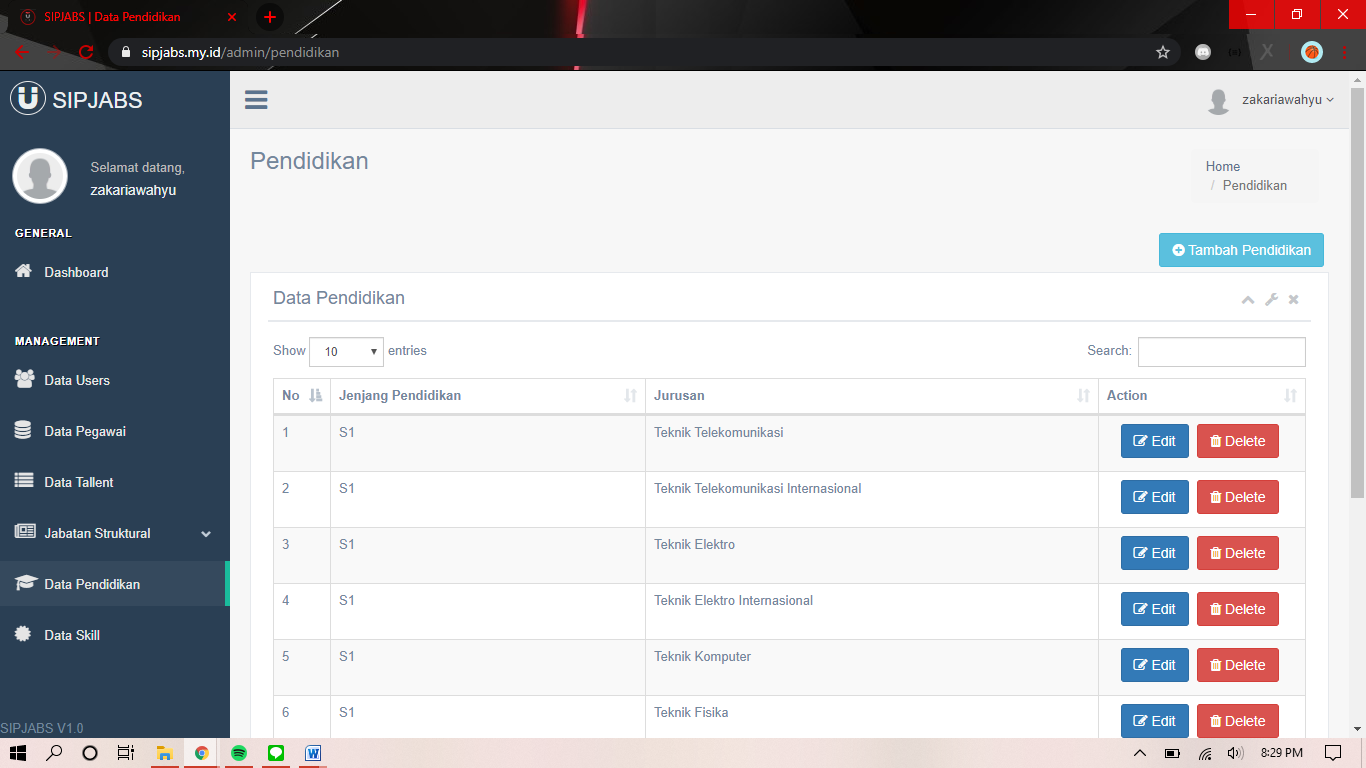
\includegraphics[width=0.8\textwidth]
		{pics/admin/implementasi/datapendidikan.png}
		\caption{Halaman Data Pendidikan - Admin}
		\label{fig:CC10}
	\end{figure}
	Gambar diatas menjelaskan data pendidikan semua pegawai Universitas Tekom, sehingga admin dapat mengetahui bahwasannya pegawai di Universitas Telkom memiliki jenjang pendidikan dan jurusan apa saja. Didapat apabila admin megklik menu “data pendidikan”.
	
	\item Halaman \textit{Edit} Pendidikan
	\begin{figure}
		\centering
		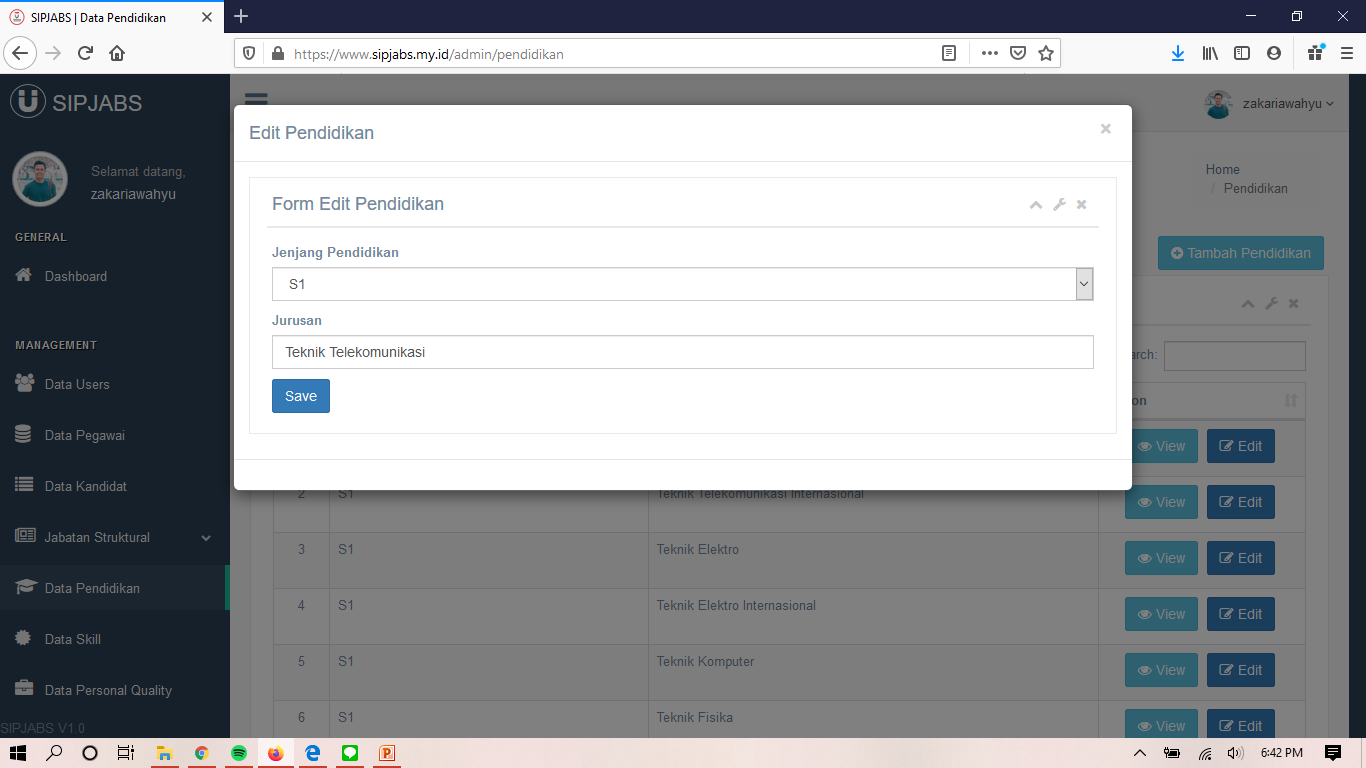
\includegraphics[width=0.8\textwidth]
		{pics/admin/implementasi/editpendidikan.png}
		\caption{Halaman \textit{Edit} Pendidikan - Admin}
		\label{fig:CC10}
	\end{figure}
	Untuk tampilan diatas adalah tampilan \textit{pop-up} dari \textit{form edit} pendidikan, apabila admin ingin mengedit data pendidikan dengan mengklik \textit{button “edit”} kemudian memilih jenjang pendidikan dan menginputkan jurusan, apabila sudah sesuai klik \textit{button “save”} untuk menyimpan data.
	
	\item Halaman Tambah Pendidikan
	\begin{figure}
		\centering
		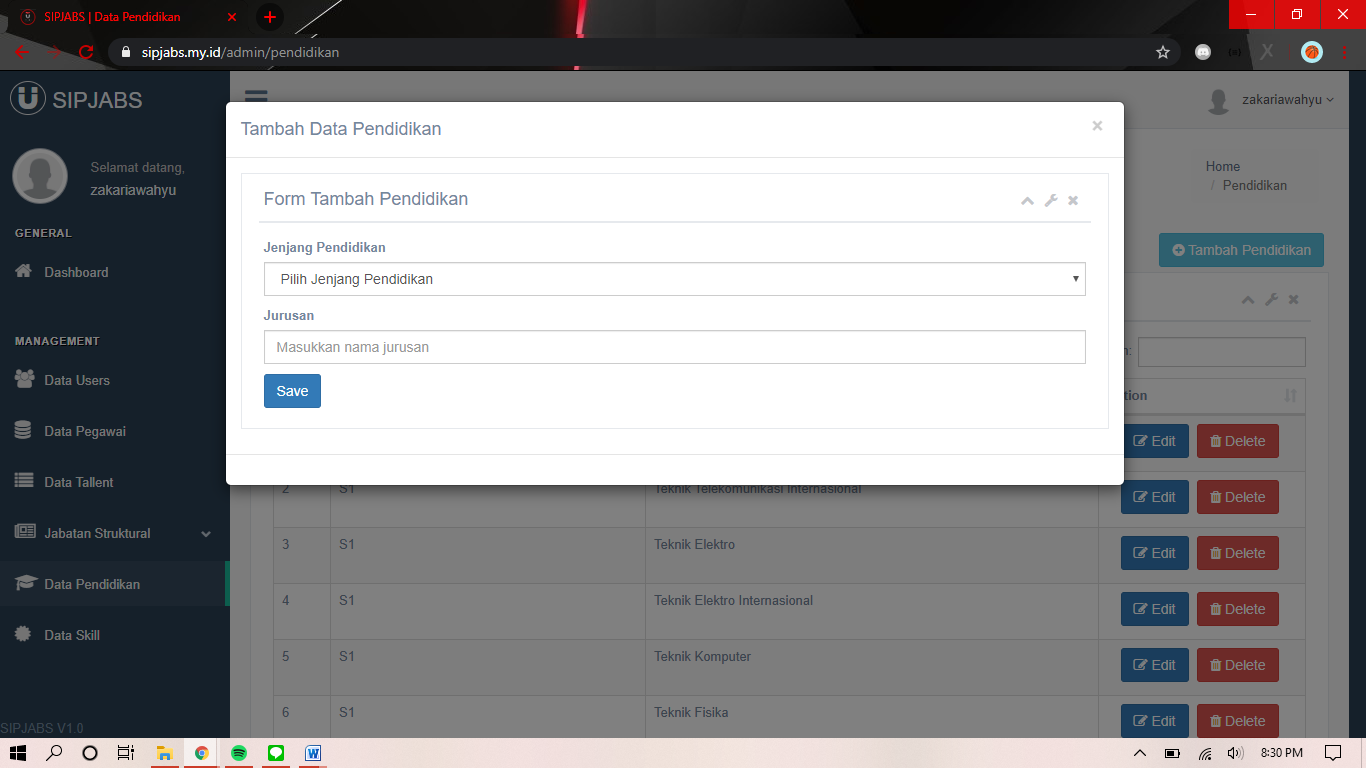
\includegraphics[width=0.8\textwidth]
		{pics/admin/implementasi/tambahpendidikan.png}
		\caption{Halaman Tambah Pendidikan - Admin}
		\label{fig:CC10}
	\end{figure}
	Gambar diatas menampilkan \textit{pop-up} tambah data pendidikan, apabila terdapat pegawai baru, namun data pendidikan belum terdaftar maka admin dapat menambahkannya dengan memilih jenjang pendidikan dan menginput jurusan,  kemudian diakhiri dengan mengklik \textit{button “save”} dan data akan tersimpan.
	
	\item Halaman Data \textit{Skill}
	\begin{figure}
		\centering
		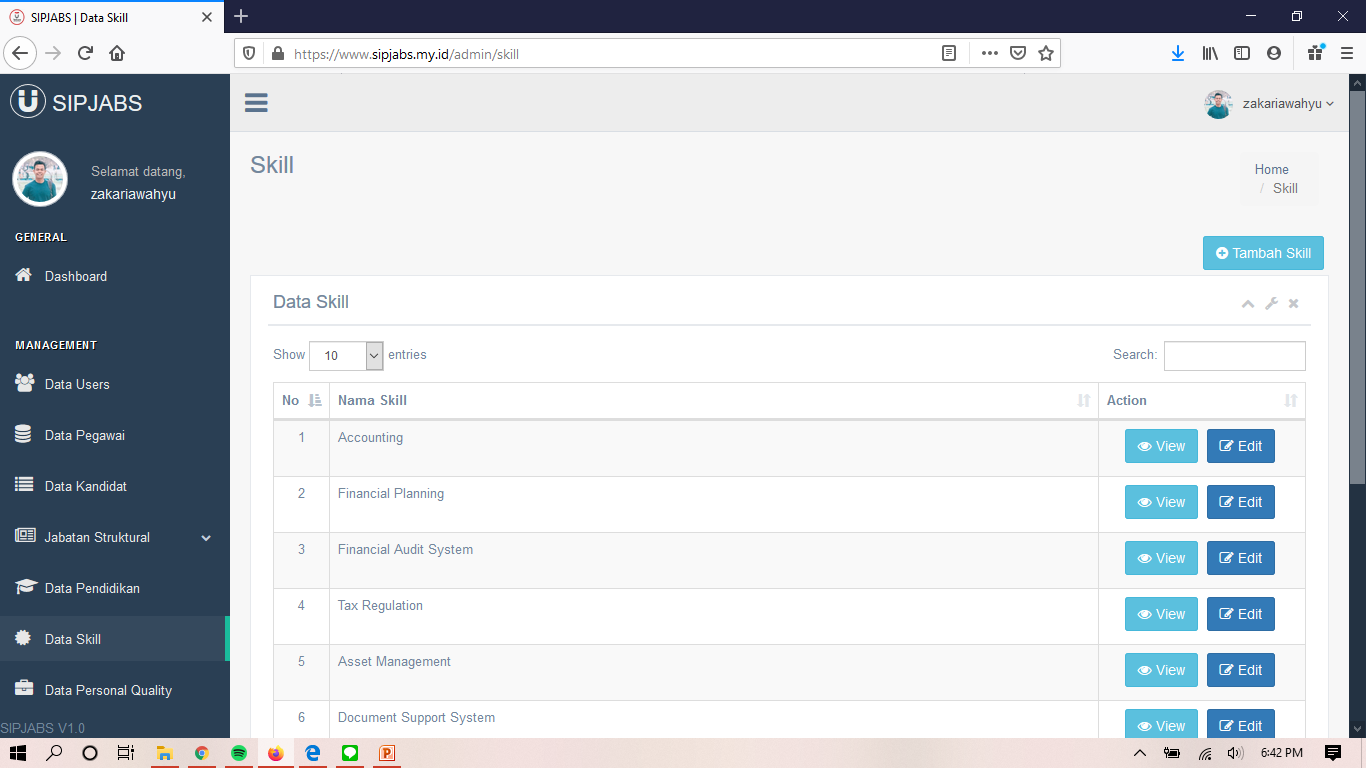
\includegraphics[width=0.8\textwidth]
		{pics/admin/implementasi/dataskill.png}
		\caption{Halaman Data \textit{Skill} - Admin}
		\label{fig:CC10}
	\end{figure}
	Gambar diatas merupakan implementasi data \textit{skill} yang ada di Universitas Telkom, data tersebut ada karena setiap pegawai memiliki \textit{skill} kemudian data \textit{skill} dari semua pegawai disatukan didalam data \textit{skill},  untuk menunjang pekerjaan. 
	
	\item Halaman \textit{Edit Skill}
	\begin{figure}
		\centering
		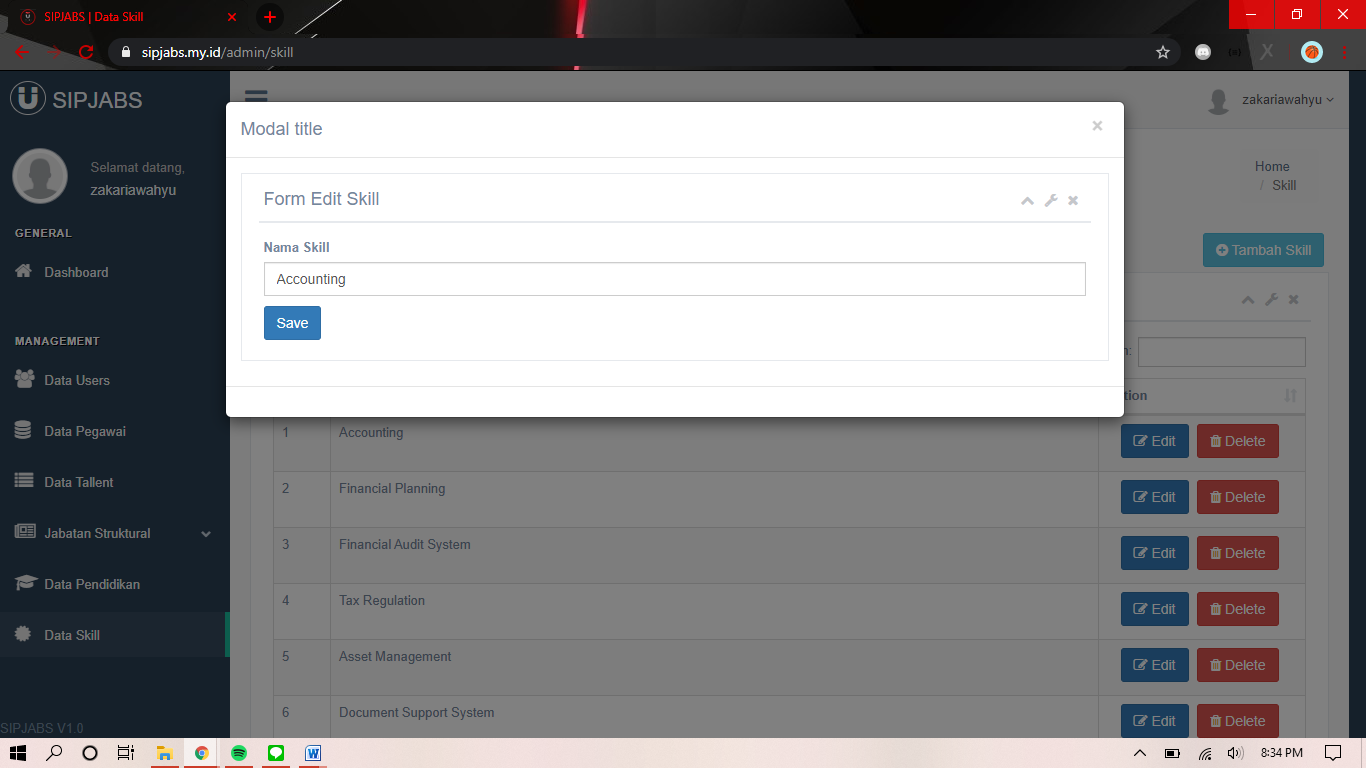
\includegraphics[width=0.8\textwidth]
		{pics/admin/implementasi/editskill.png}
		\caption{Halaman \textit{Edit Skill} - Admin}
		\label{fig:CC10}
	\end{figure}
	Implementasi diatas menampikan \textit{pop-up form edit skill}, dimana admin dapat mengedit nama \textit{skill} menjadi lebih sesuai, dan menyimpannya kembali dengan mengklik \textit{button “save”}.
	
	\item Halaman Tambah Skill
	\begin{figure}
		\centering
		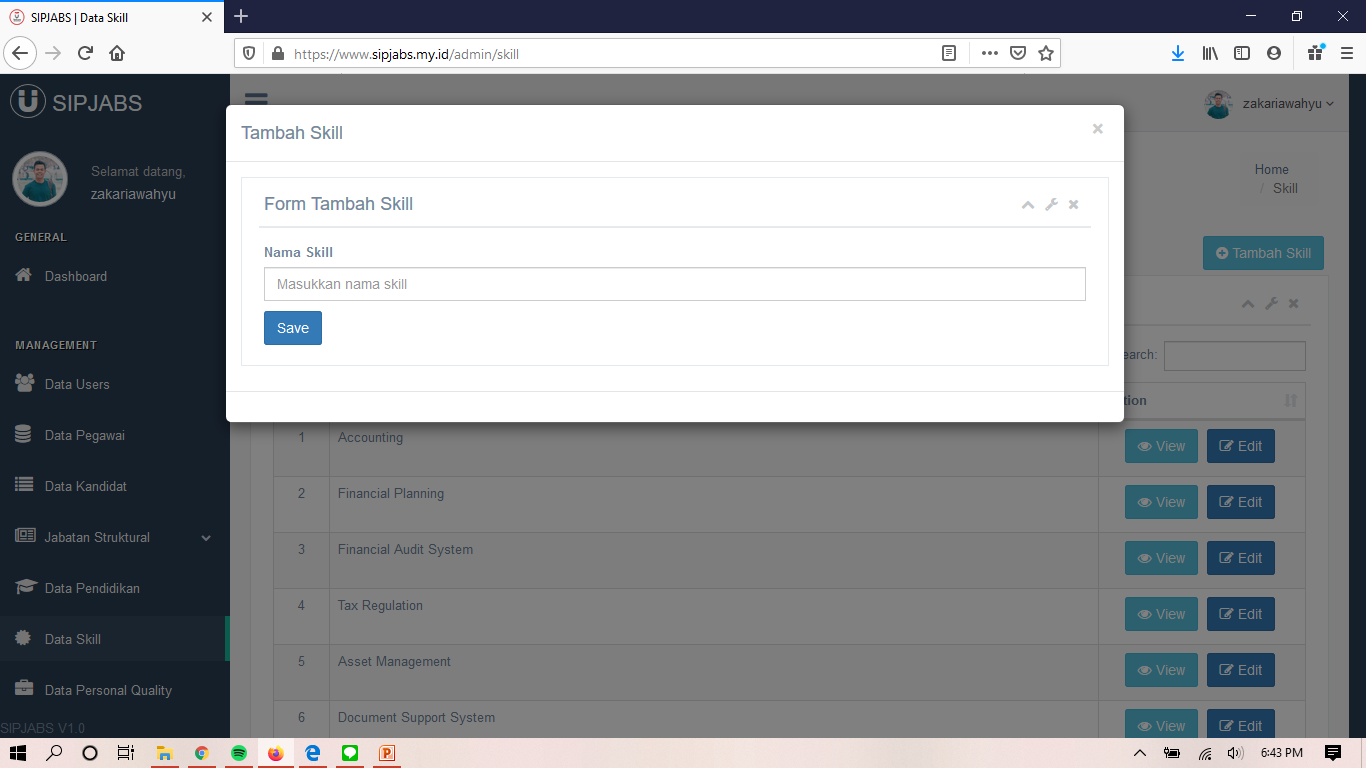
\includegraphics[width=0.8\textwidth]
		{pics/admin/implementasi/tambahskill.png}
		\caption{Halaman Tambah Skill - Admin}
		\label{fig:CC10}
	\end{figure}
	Untuk tampilan diatas adalah tambah data \textit{skill}, admin dapat menambahkan data \textit{skill} dengan mengkil button “tambah \textit{skill}” apabila \textit{skill} pada pegawai belum terdaftar pada data \textit{skill}, lalu inputkan nama \textit{skill} dan menyimpannya dengan klik \textit{button “save”}.
	
	\newpage
	\item Halaman Data \textit{Personal Quality}
	\begin{figure}
		\centering
		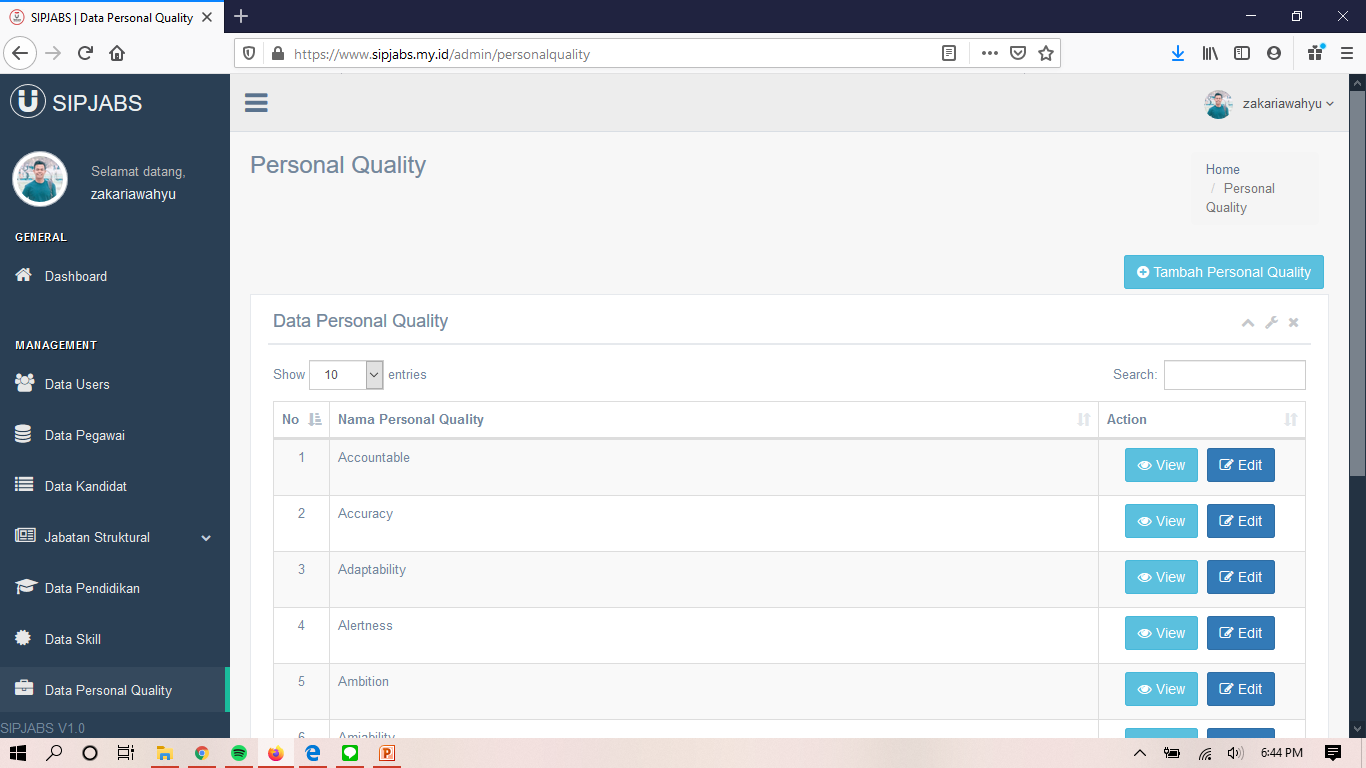
\includegraphics[width=0.8\textwidth]
		{pics/admin/implementasi/datapersonalquality.png}
		\caption{Halaman Data \textit{Personal Quality} - Admin}
		\label{fig:CC10}
	\end{figure}
	Gambar diatas merupakan implementasi data \textit{personal quality} yang ada di Universitas Telkom, data tersebut ada karena setiap pegawai memiliki \textit{personal quality} kemudian data \textit{skill} dari semua pegawai disatukan didalam data \textit{personal quality},  untuk menunjang pekerjaan. 
	
	\item Halaman \textit{Edit Personal Quality}
	\begin{figure}
		\centering
		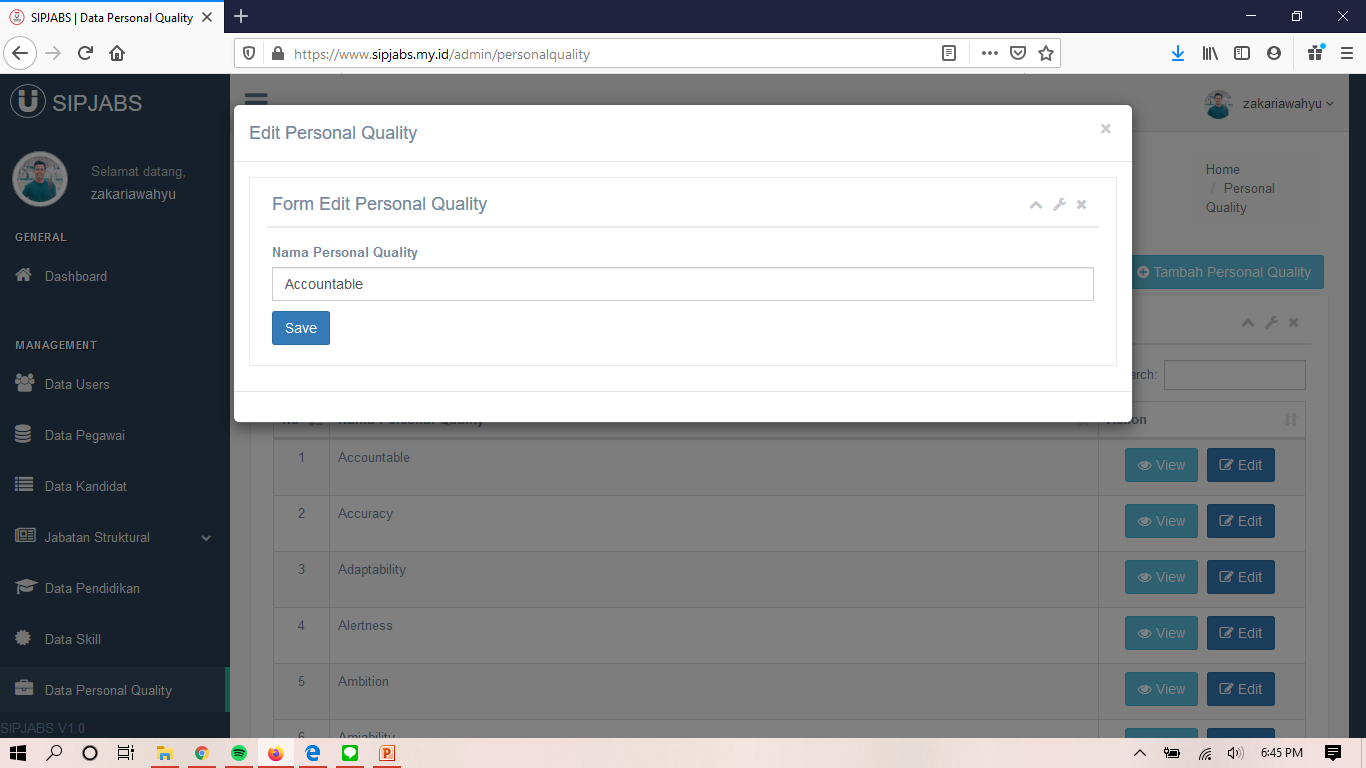
\includegraphics[width=0.8\textwidth]
		{pics/admin/implementasi/editpersonalquality.png}
		\caption{Halaman \textit{Edit Personal Wuality} - Admin}
		\label{fig:CC10}
	\end{figure}
	Implementasi diatas menampikan \textit{pop-up form edit personal quality}, dimana admin dapat mengedit nama \textit{personal quality} menjadi lebih sesuai, dan menyimpannya kembali dengan mengklik \textit{button “save”}.
	
	\newpage
	\item Halaman Tambah Personal Quality
	\begin{figure}
		\centering
		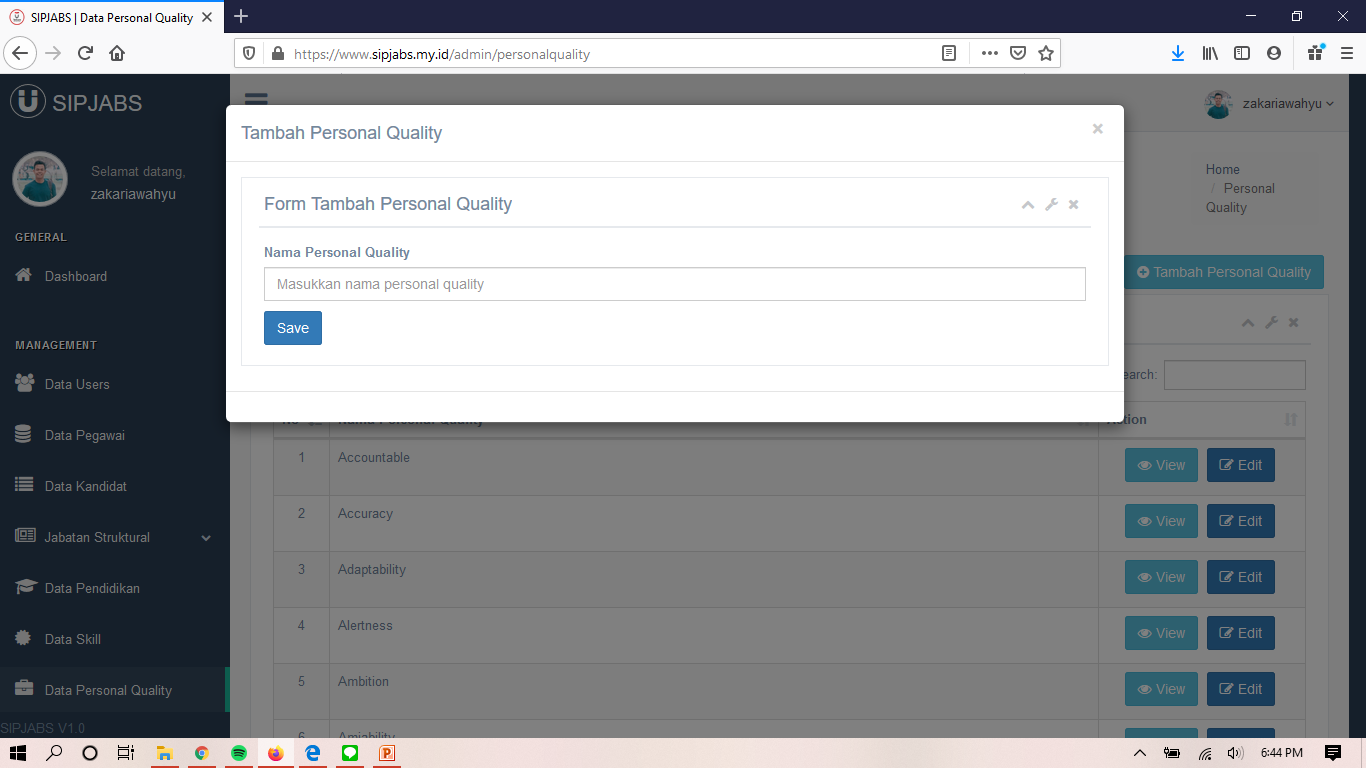
\includegraphics[width=0.8\textwidth]
		{pics/admin/implementasi/tambahpersonalquality.png}
		\caption{Halaman Tambah Personal Quality - Admin}
		\label{fig:CC10}
	\end{figure}
	Untuk tampilan diatas adalah tambah data \textit{personal quality}, admin dapat menambahkan data \textit{personal quality} dengan mengkil button “tambah \textit{personal quality}”.
	
\end{enumerate}

\subsubsection{Implementasi \textit{User}}

\begin{enumerate}
	
	\item Halaman \textit{Login}
	\begin{figure}
		\centering
		\includegraphics[width=0.8\textwidth]
		{pics/user/implementasi/login.png}
		\caption{Halaman \textit{Login User}}
		\label{fig:CC10}
	\end{figure}
	
	Tampilan diatas merupakan implementasi dari BAB III dimana \textit{user} harus menginputkan \textit{username} dan \textit{password} untuk dapat melanjutkan penggunaan aplikasi, apabila sudah diinputkan lanjut untuk mengklik \textit{button “login”}. 
	
	\item Halaman \textit{Dashboard}
	\begin{figure}
		\centering
		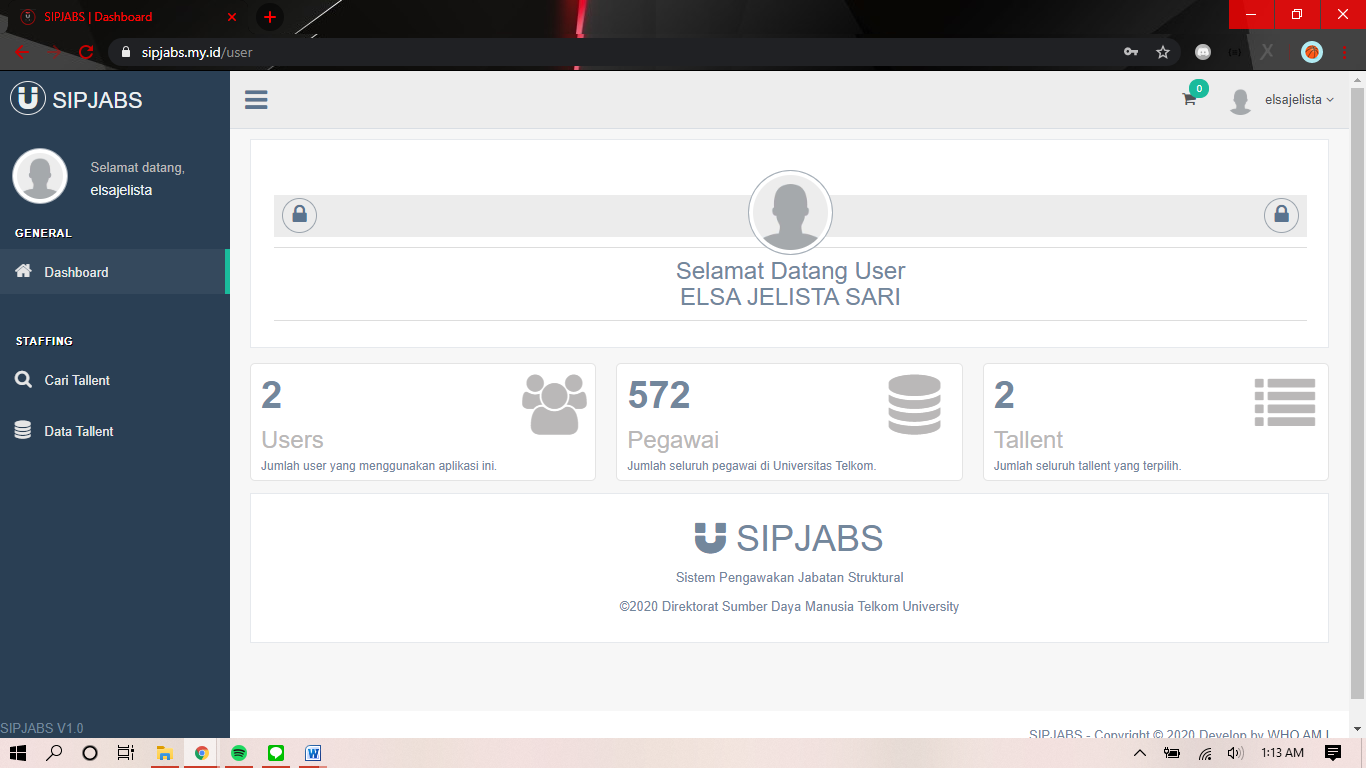
\includegraphics[width=0.8\textwidth]
		{pics/user/implementasi/dashboard.png}
		\caption{Halaman \textit{Dashboard User}}
		\label{fig:CC10}
	\end{figure}
	
	Gambar diatas mengimplementasikan isi dari \textit{dashboard user}, berbeda dengan \textit{dashboard} yang dimiliki admin, \textit{dashboard user} hanya menampilkan jumlah \textit{user} yang dapat mengakses aplikasi \textbf{SiPJabS}, jumlah pegawai yang terdaftar di Universitas Telkom, serta jumlah kandidat yang sudah dipilih. 
	
	\item Halaman \textit{Profile}
	\begin{figure}
		\centering
		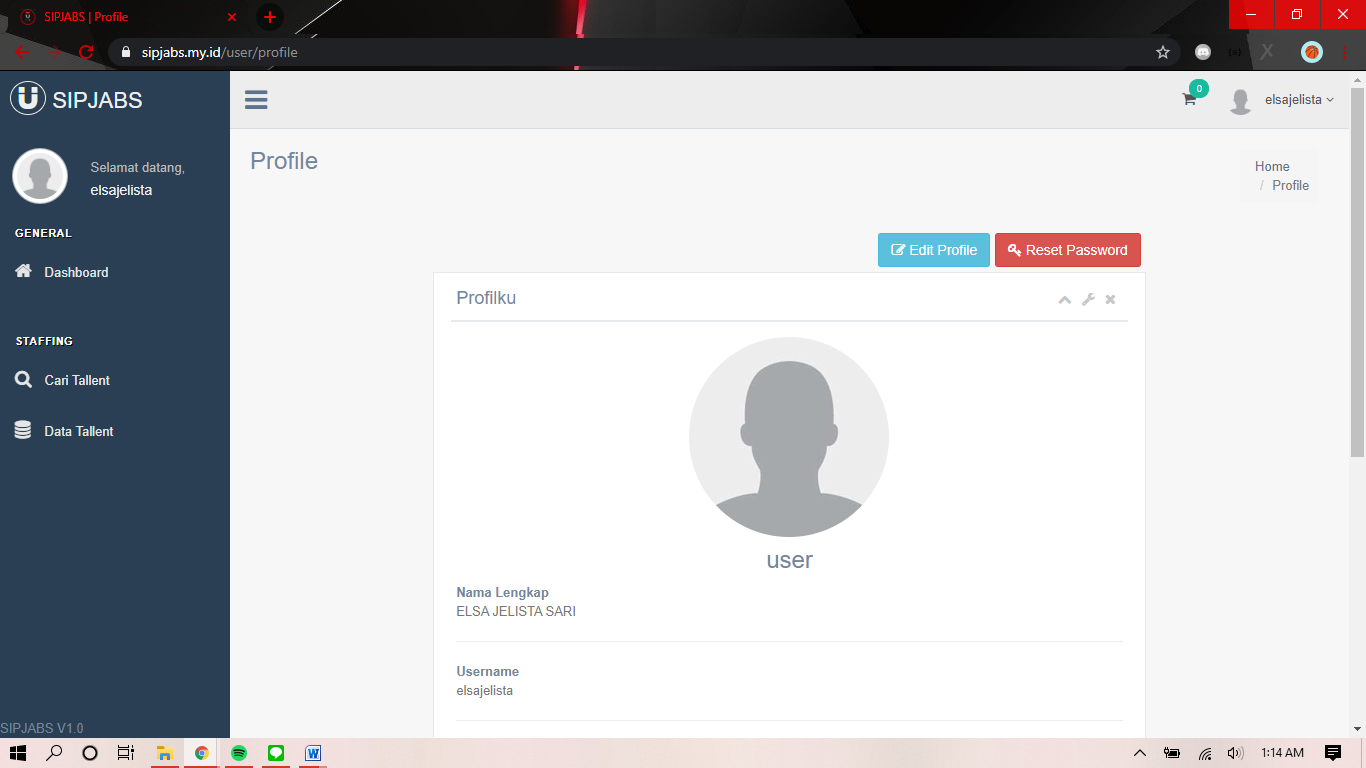
\includegraphics[width=0.8\textwidth]
		{pics/user/implementasi/profile.png}
		\caption{Halaman \textit{Profile User}}
		\label{fig:CC10}
	\end{figure}
	
	Implementasi diatas menunjukkan isi \textit{profile} dari \textit{user}, terdapat nama lengkap, \textit{username}, email, status pegawai, unit kerja, jabatan, dan NIP. Admin dapat membuka halaman tersebut dengan cara klik \textit{username} yang ada di atas kanan, kemudian akan terdapat \textit{dropdown} dan klik \textit{profile}, maka halaman akan tampil seperti diatas. 
	
	\item Halaman \textit{Edit Profile}
	\begin{figure}
		\centering
		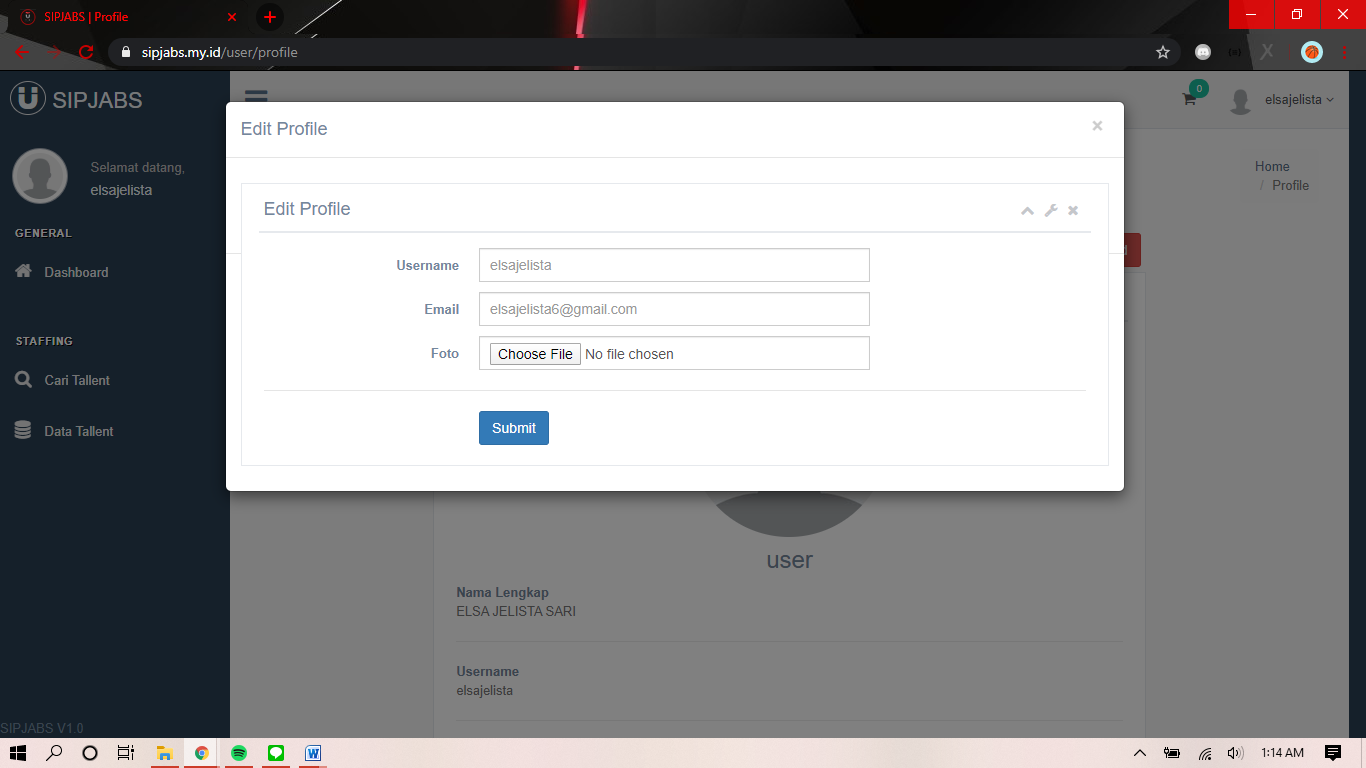
\includegraphics[width=0.8\textwidth]
		{pics/user/implementasi/editprofile.png}
		\caption{Halaman \textit{Edit Profile User}}
		\label{fig:CC10}
	\end{figure}
	
	Gambar diatas mengimplementasikan\textit{ edit profile user} dengan \textit{pop-up}, \textit{user} dapat mengganti \textit{username}, email atau foto. Kemudian klik “\textit{submit}” untuk menyimpan data yang sudah diganti agar tersimpan.
	
	\item Halaman \textit{Reset Password}
	\begin{figure}
		\centering
		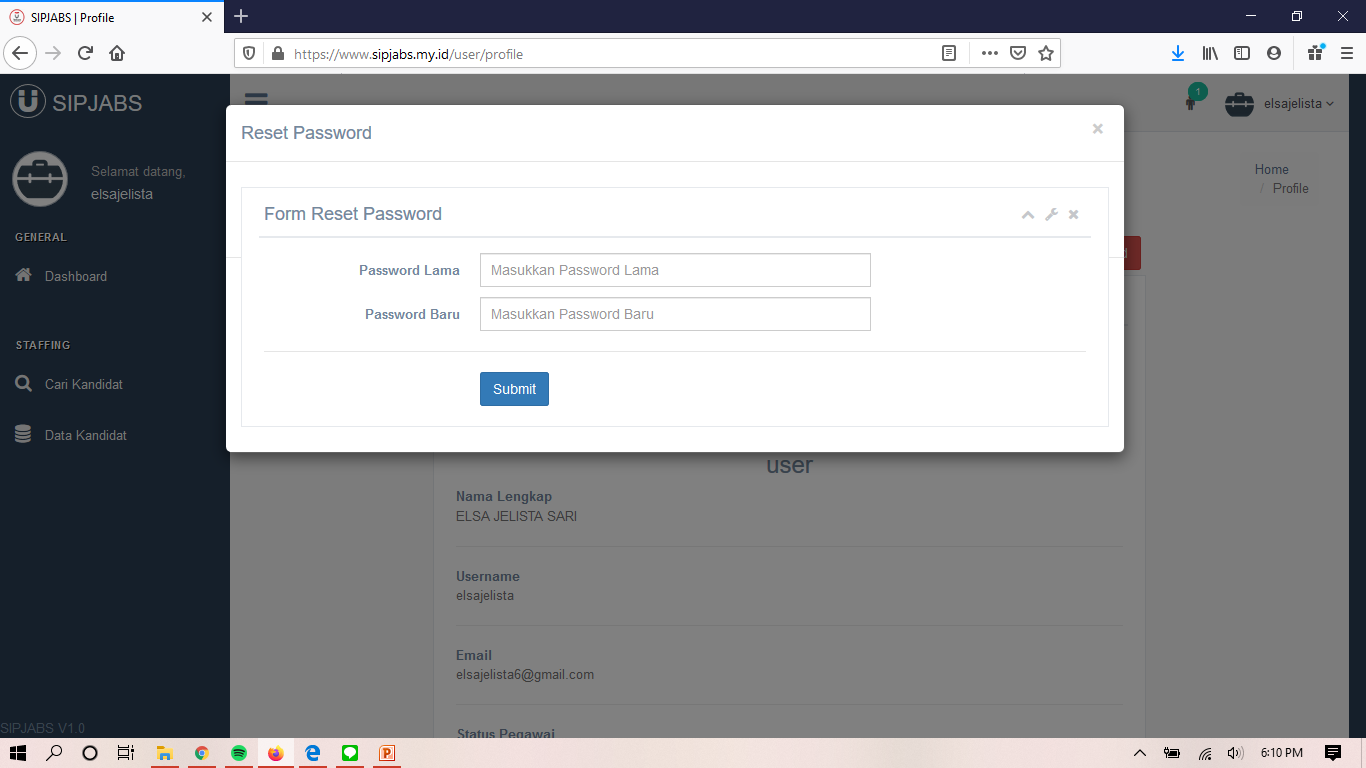
\includegraphics[width=0.8\textwidth]
		{pics/user/implementasi/resetpassword.png}
		\caption{Halaman \textit{Reset Password User}}
		\label{fig:CC10}
	\end{figure}
	
	Implementasi diatas menjelaskan bahwasannya \textit{user} dapat mengganti \textit{passsword}, apabila \textit{password} tersebut sudah diketahui oleh pihak lain, \textit{user} dapat mengklik \textit{button “reset password”} kemudian akan tampil\textit{ pop-up} seperti diatas, \textit{user} harus menginputkan \textit{password} lama dan \textit{password} yang baru, lalu klik “\textit{submit}” untuk menyimpan \textit{password} yang baru.
	
	\item Halaman \textit{Help}
	\begin{figure}
		\centering
		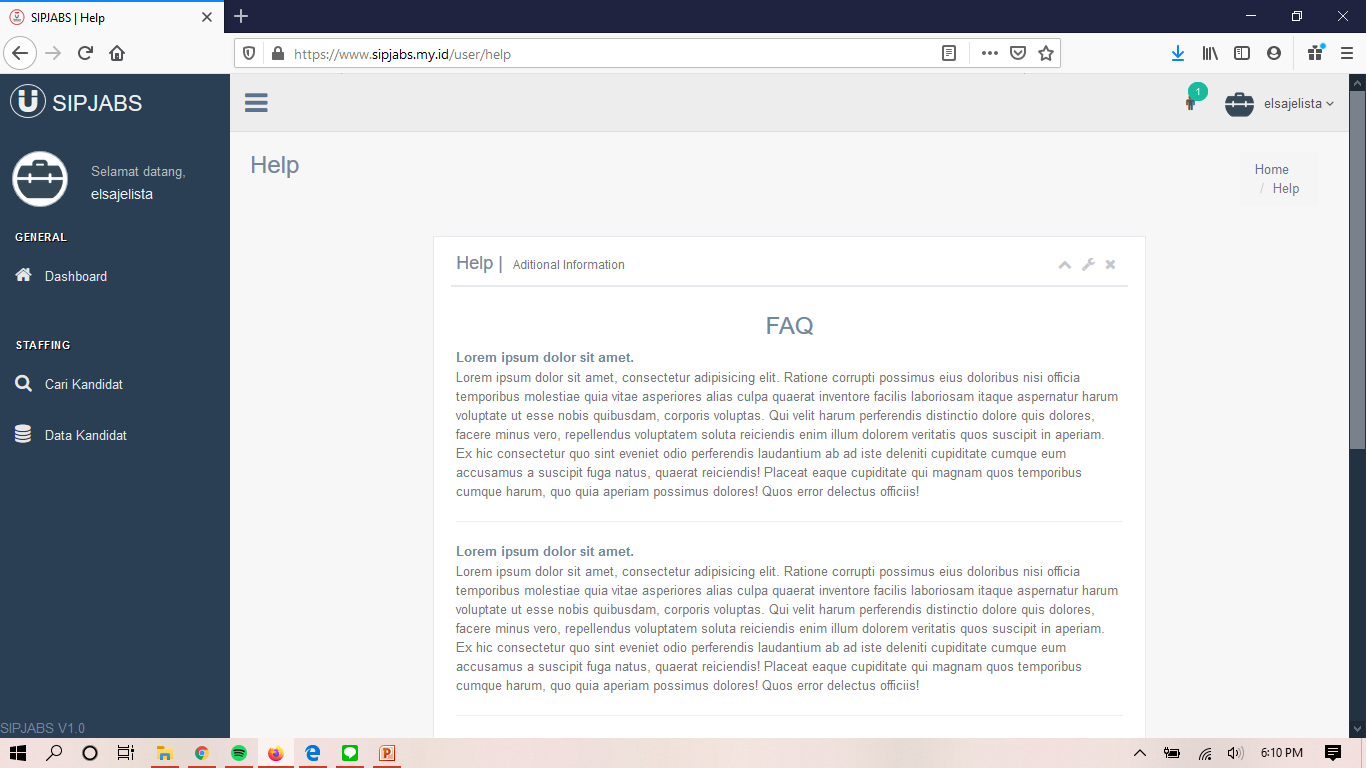
\includegraphics[width=0.8\textwidth]
		{pics/user/implementasi/help.png}
		\caption{Halaman \textit{Help User}}
		\label{fig:CC10}
	\end{figure}

	\item Halaman Cari Kandidat
	\begin{figure}
		\centering
		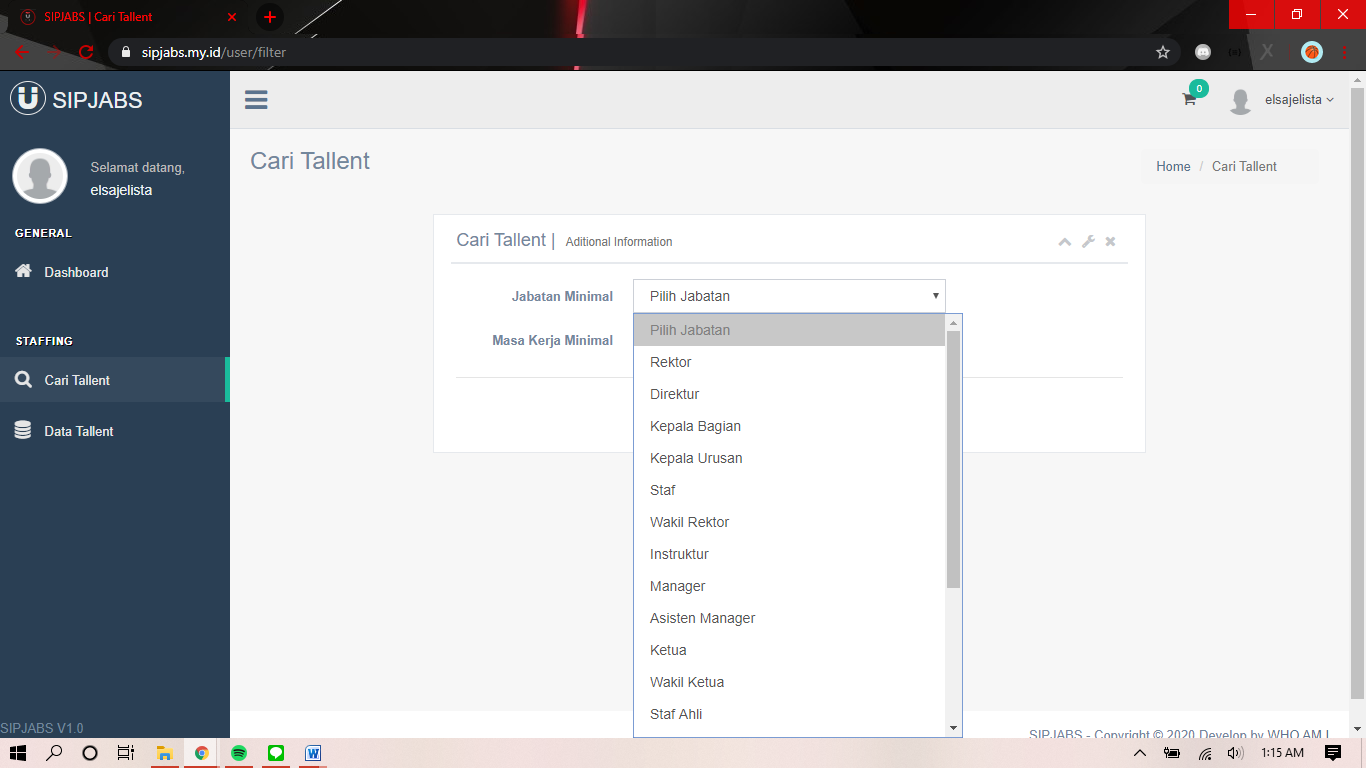
\includegraphics[width=0.8\textwidth]
		{pics/user/implementasi/caritallent.png}
		\caption{Halaman Cari Kandidat - User}
		\label{fig:CC10}
	\end{figure}
	
	Gambar diatas mengimplementasikan apabila \textit{user} ingin mencari kandidat yang dibutuhkan sesuai \textit{requirement} perusahaan untuk menggantikan atau mengisi posisi yang kosong, dengan cara klik “cari kandidat” pada menu, lalu akan muncul halaman seperti diatas, user harus memilih jabatan yang dituju, jabatan  minimal yang dibutuhkan dan menginputkan masa kerja. Dan klik \textit{button} “cari”.
	
	\newpage
	\item Halaman \textit{Filtering}
	\begin{figure}
		\centering
		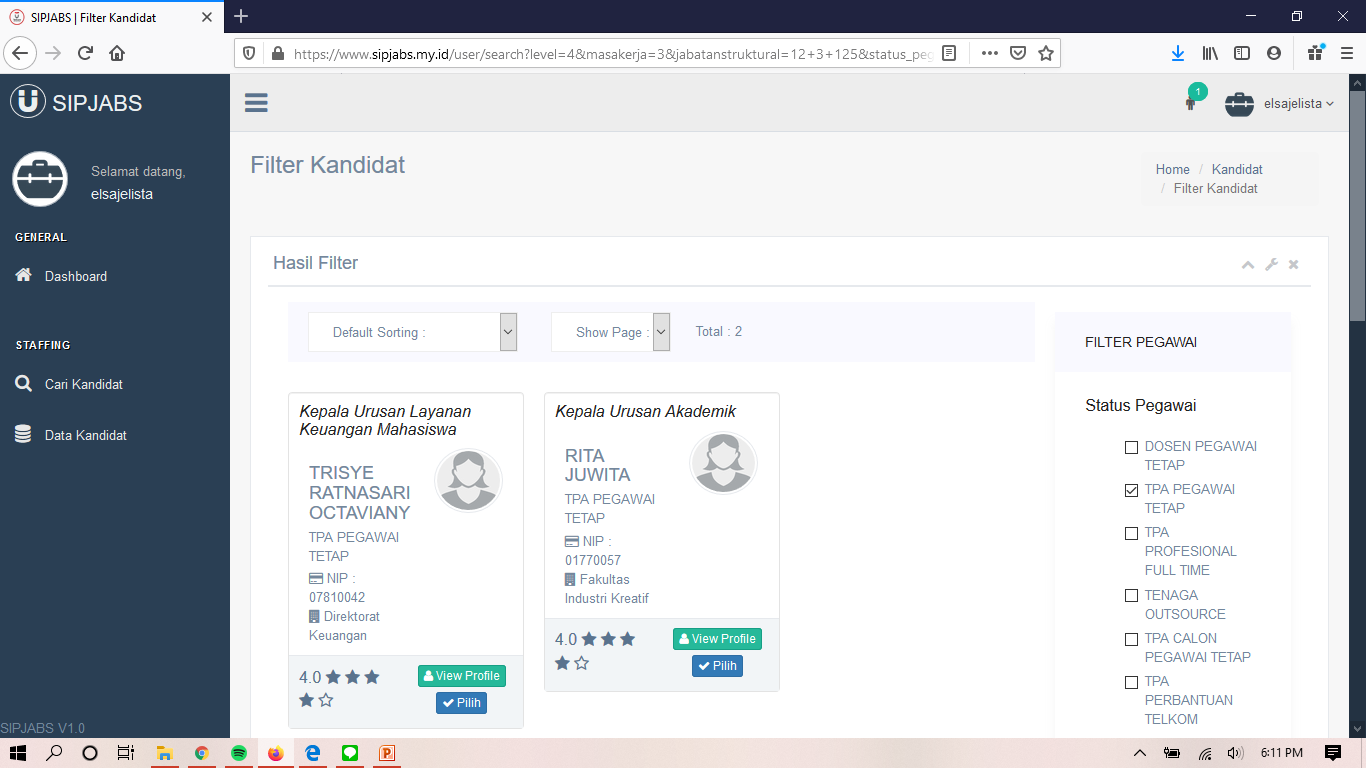
\includegraphics[width=0.8\textwidth]
		{pics/user/implementasi/hasiltallent.png}
		\caption{Halaman \textit{Filtering - User}}
		\label{fig:CC10}
	\end{figure}
	
	Implementasi diatas menampilkan data kandidat yang tersedia, kemudian \textit{user} dapat menyeleksi kembali dengan memilih \textit{filter} pegawai, jenjang pendidikan, jurusan dan \textit{skill} yang dimiliki oleh pegawai.
	
	\item Halaman\textit{ View Detail} Pegawai
	\begin{figure}
		\centering
		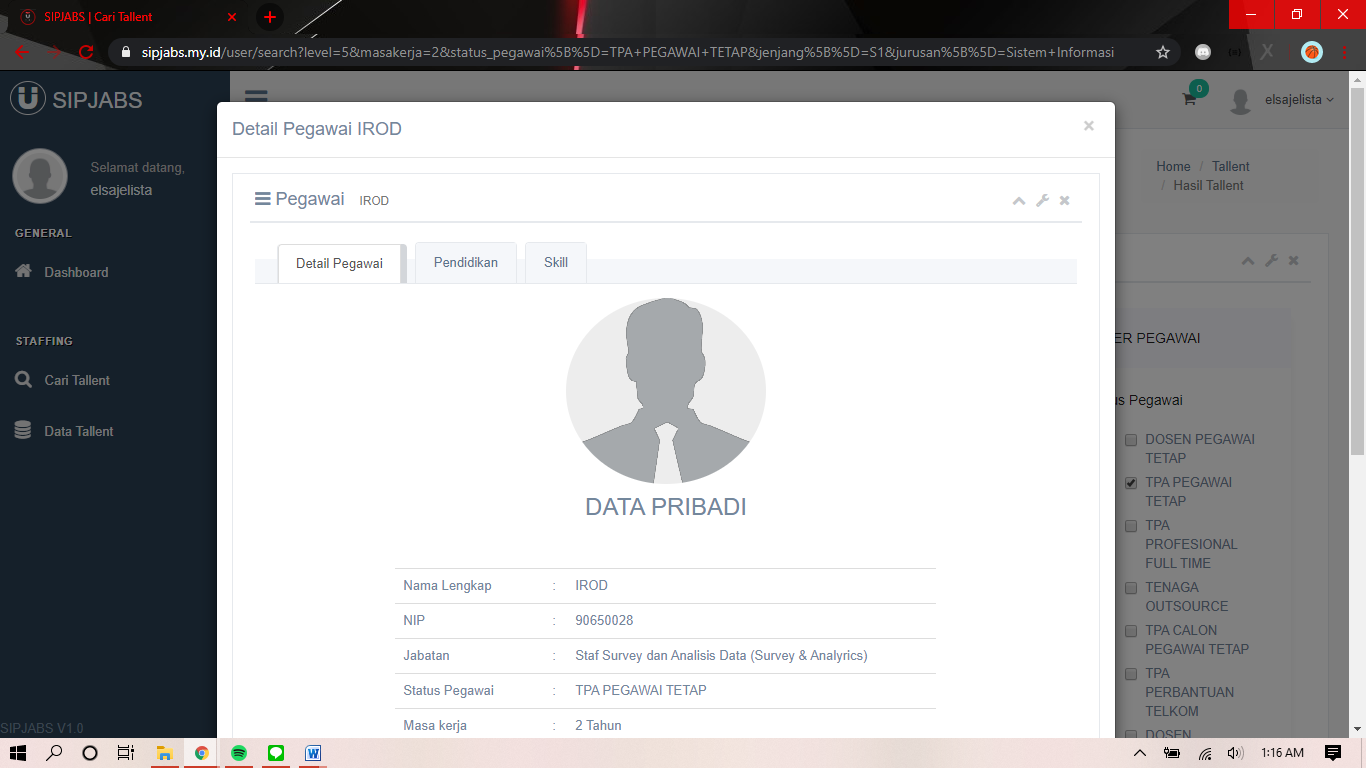
\includegraphics[width=0.8\textwidth]
		{pics/user/implementasi/viewdetailpegawai.png}
		\caption{Halaman \textit{View Detail} Pegawai - \textit{User}}
		\label{fig:CC10}
	\end{figure}
	
	Gambar diatas mengimpementasikan bahwasannya \textit{user} dapat melihat data pribadi yang dimiliki kandidat, dengan cara klik\textit{ button “view”} maka akan tampil halaman seperti diatas dan menampilkan data pribadi pegawai beserta data riwayat pendidikan, skill dan personal quality.
	
	\newpage
	\item Halaman Kandidat Sementara
	\begin{figure}
		\centering
		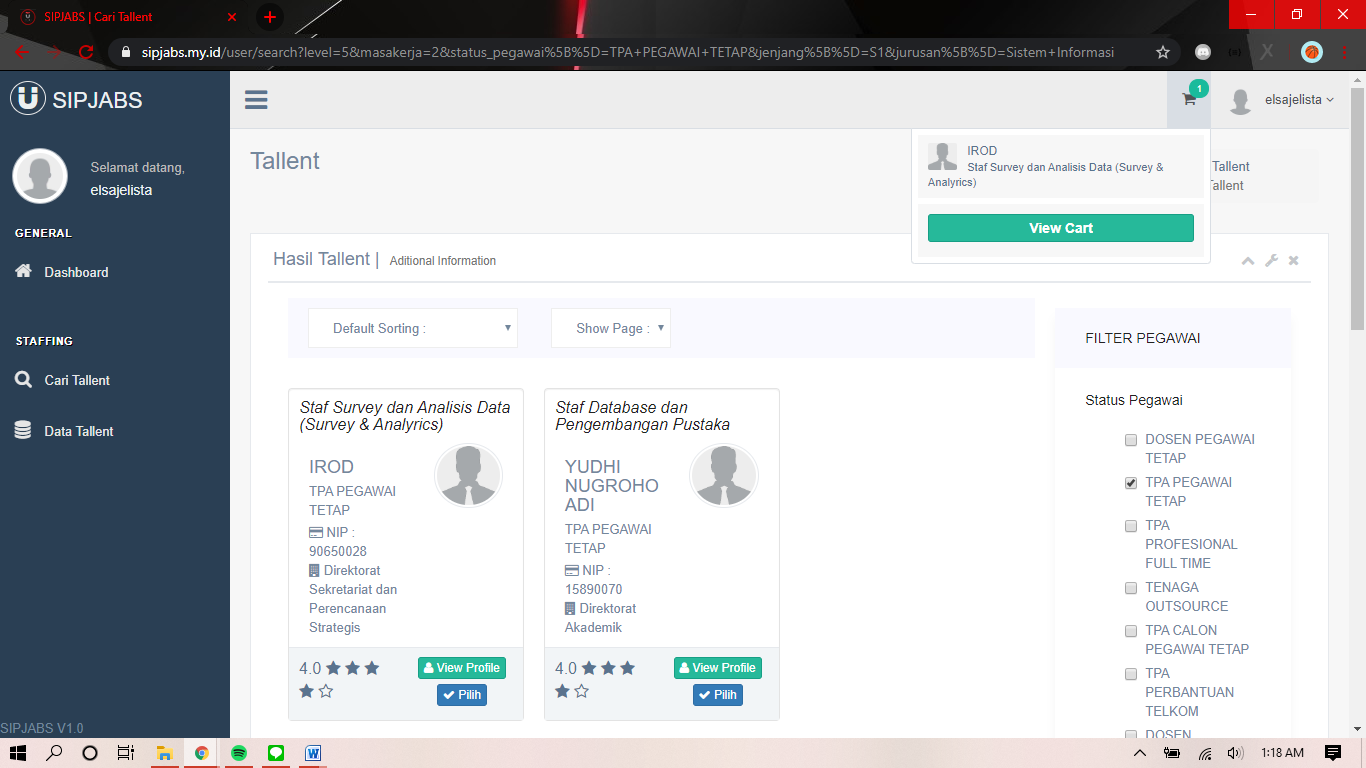
\includegraphics[width=0.8\textwidth]
		{pics/user/implementasi/cartuser.png}
		\caption{Halaman \textit{Cart - User}}
		\label{fig:CC10}
	\end{figure}
	
	Gambar diatas menjelaskan bahwasannya \textit{user} sudah memilih kandidat yang sesuai dengan yang dibutuhkan untuk mengganti atau mengisi posisi yang kosong.  
	
	\item Halaman \textit{View} Kandidat Sementara
	\begin{figure}
		\centering
		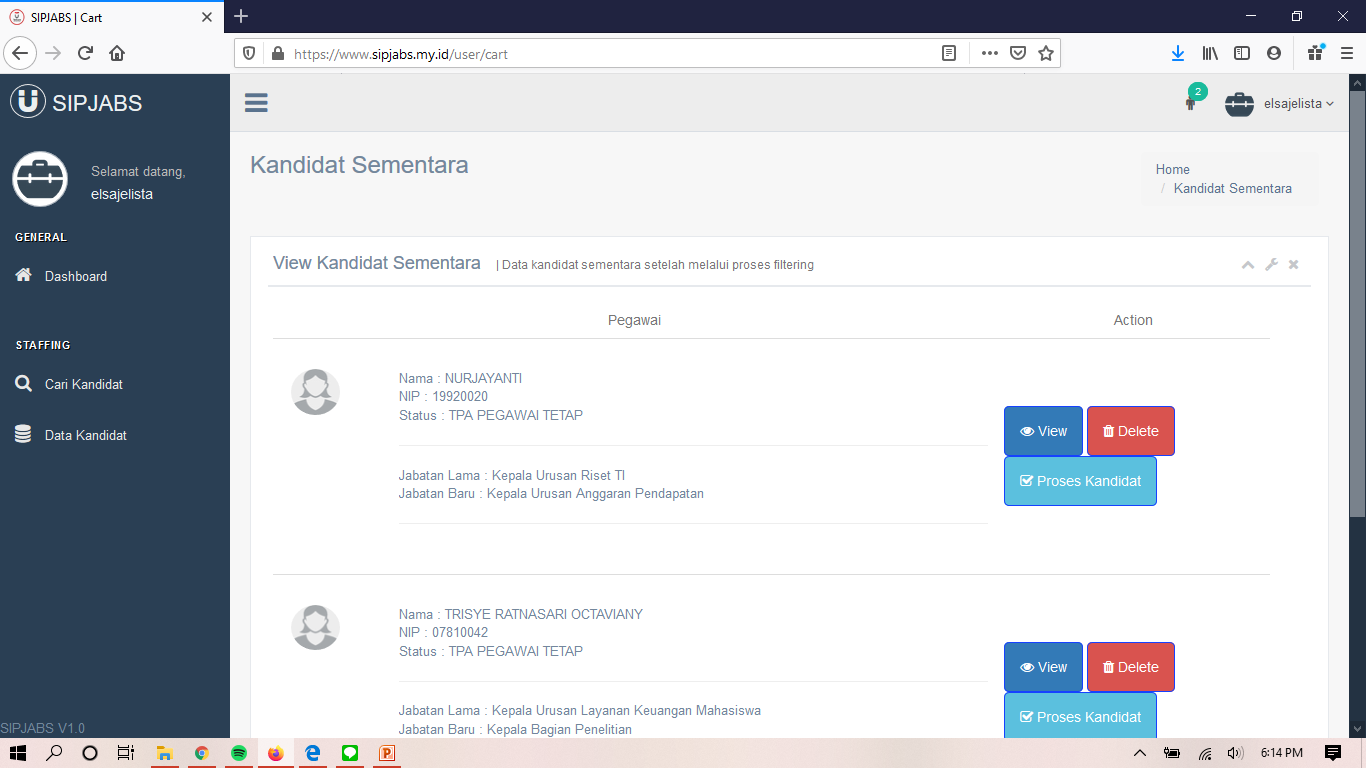
\includegraphics[width=0.8\textwidth]
		{pics/user/implementasi/viewcart.png}
		\caption{Halaman \textit{View} Kandidat Sementara}
		\label{fig:CC10}
	\end{figure}
	
	Gambar diatas mengimplementasikan halaman \textit{view }pada kandidat sementara, apabila \textit{user} telah memilih kandidat maka data tersebut akan masuk kedalam kandidat sementara, sebelum diproses ke data kandidat. 
	
	\newpage
		\item Halaman Data Kandidat
	\begin{figure}
		\centering
		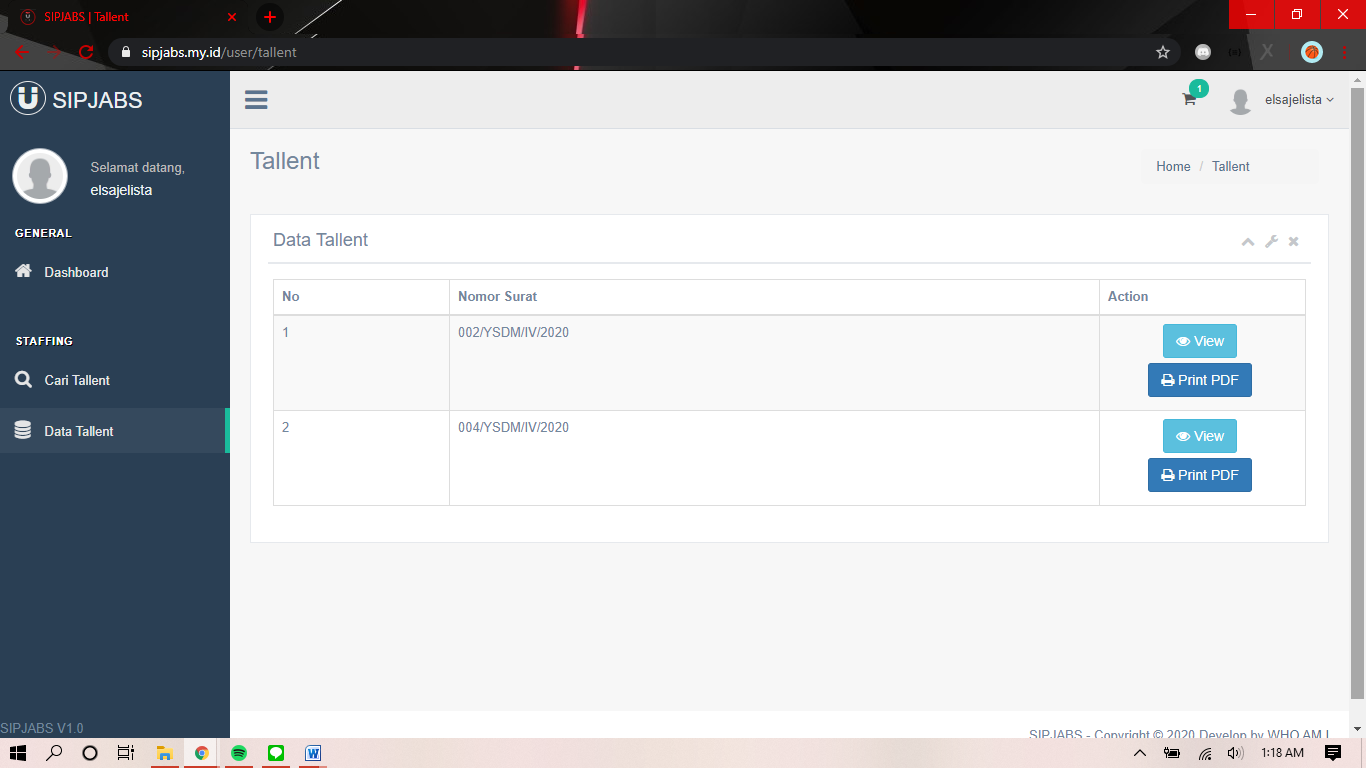
\includegraphics[width=0.8\textwidth]
		{pics/user/implementasi/datatallent.png}
		\caption{Halaman Data Kandidat}
		\label{fig:CC10}
	\end{figure}
	
	Gambar diatas mengimplementasikan isi dari  data kandidat yang dimiliki \textit{user}, data tersebut sudah dipilih sesuai dengan \textit{requirement} perusahaan dan sesuai dengan \textit{job descripton} yang dimiliki pegawai dan selanjutka anak diajukan untuk penilaian.
	
\end{enumerate}

\subsection{Struktur Kode}
Struktur kode merupakan kumpulan kode atau script yang berfungsi untuk menjalankan setiap perintah dalam setiap proses pembuatan aplikasi. Berikut struktur kode yang ada pada aplikasi SiPJabS:

\begin{table}
	\caption{Tabel Struktur Kode}
	\centering
	\begin{tabular}{ | l | l | p{20mm} | p{22mm} | p{47mm} |}
		\hline
		
		\textbf{No} & \textbf{Struktur Kode} & \textbf{Controller} & \textbf{Method} & \textbf{Deskripsi}  \\
		\hline
		
		
		\multirow{4}{*}{1} &  \multirow{4}{*}{User} & \multirow{4}{20mm}{} & index() &  \multirow{4}{47mm}{Berfungsi untuk melakukan proses menampilkan, menambah dan menghapus data kandidat sementara } \\
		& & Cart & show() & \\
		& & Controller & destroy() & \\
		& & & addCart() & \\
		\hline
		
		\multirow{5}{*}{2} &  \multirow{5}{*}{User} & \multirow{5}{20mm}{} & index() &  \multirow{5}{47mm}{Berfungsi untuk melakukan proses filtering pegawai untuk mencari kandidat berdasarkan requirement} \\
		& & Filter & show() & \\
		& & Controller & filterTallent() & \\
		& & & getJabatan() & \\
		& & & fetch() & \\
		\hline
		
		
	\end{tabular}
\end{table}

\newpage

\begin{table}
	\centering
		\caption{Tabel Struktur Kode (1)}
	\begin{tabular}{ | l | l | p{20mm} | p{22mm} | p{47mm} |}
		\hline
		
		\textbf{No} & \textbf{Struktur Kode} & \textbf{Controller} & \textbf{Method} & \textbf{Deskripsi}  \\
		\hline
		
		
		\multirow{5}{*}{3} &  \multirow{5}{*}{User} & \multirow{5}{20mm}{} & index() &  \multirow{5}{47mm}{Berfungsi untuk melakukan proses melihat profile akun, reset password dan edit profile pada user } \\
		& & Profile & show() & \\
		& & Controller & edit() & \\
		& & & update() & \\
		& & & resetPass() & \\
		\hline
		
		\multirow{5}{*}{4} &  \multirow{5}{*}{User} & \multirow{5}{20mm}{} & index() &  \multirow{5}{47mm}{Berfungsi untuk melakukan pengelolaan seperti menambahkan data kandidat terpilih, menghapus dan print pdf} \\
		& & Tallent & show() & \\
		& & Controller & destroy() & \\
		& & & cetak pdf() & \\
		& & & addTallent() & \\
		\hline
		
		5 & User & User Controller & index() & Berfungsi menampilkan halaman dashboard user \\
		\hline
		
		6 & Admin & Admin Controller & index() & Berfungsi menampilkan halaman dashboard admin \\
		\hline
		
		\multirow{6}{*}{7} &  \multirow{6}{*}{Admin} & \multirow{6}{20mm}{} & index() &  \multirow{6}{47mm}{Berfungsi untuk melakukan proses CRUD pada jabatan} \\
		& &  & create() & \\
		& & Jabatan & store() & \\
		& & Controller& show() & \\
		& & & edit() & \\
		& & & update() & \\
		\hline
		
		\multirow{6}{*}{8} &  \multirow{6}{*}{Admin} & \multirow{6}{20mm}{} & index() &  \multirow{6}{47mm}{Berfungsi untuk melakukan proses CRUD pada jabatan struktural} \\
		& & Jabatan  & create() & \\
		& & Struktural & store() & \\
		& & Controller& show() & \\
		& & & edit() & \\
		& & & update() & \\
		\hline
		
		\multirow{6}{*}{9} &  \multirow{6}{*}{Admin} & \multirow{6}{20mm}{} & index() &  \multirow{6}{47mm}{Berfungsi untuk melakukan proses CRUD pada pegawai} \\
		& &  & create() & \\
		& & Pegawai & store() & \\
		& & Controller& show() & \\
		& & & edit() & \\
		& & & update() & \\
		\hline
		
	\end{tabular}
\end{table}

\begin{table}
	\centering
	\caption{Tabel Struktur Kode (2)}
	\begin{tabular}{ | l | l | p{20mm} | p{22mm} | p{47mm} |}
		\hline
		
		\textbf{No} & \textbf{Struktur Kode} & \textbf{Controller} & \textbf{Method} & \textbf{Deskripsi}  \\
		\hline
		
		\multirow{6}{*}{10} &  \multirow{6}{*}{Admin} & \multirow{6}{20mm}{} & index() &  \multirow{6}{47mm}{Berfungsi untuk melakukan proses CRUD pada pendidikan} \\
		& &  & create() & \\
		& & Pendidikan & store() & \\
		& & Controller& show() & \\
		& & & edit() & \\
		& & & update() & \\
		\hline
		
		\multirow{6}{*}{11} &  \multirow{6}{*}{Admin} & \multirow{6}{20mm}{} & index() &  \multirow{6}{47mm}{Berfungsi untuk melakukan proses CRUD pada personal quality} \\
		& & Personal  & create() & \\
		& & Quality & store() & \\
		& & Controller& show() & \\
		& & & edit() & \\
		& & & update() & \\
		\hline
		
		\multirow{5}{*}{12} &  \multirow{5}{*}{Admin} & \multirow{5}{20mm}{} & index() &  \multirow{5}{47mm}{Berfungsi untuk melakukan proses melihat profile akun, reset password dan edit profile pada admin} \\
		& & Profile & show() & \\
		& & Controller& edit() & \\
		& & & update() & \\
		& & & resetPass() & \\
		\hline
		
		\multirow{4}{*}{13} &  \multirow{4}{*}{Admin} & \multirow{4}{20mm}{} & index() &  \multirow{4}{47mm}{Berfungsi untuk melakukan proses menampilkan, delete dan cetak pdf kandidat } \\
		& & Tallent& show() & \\
		& & Controller& destroy() & \\
		& & & cetak pdf() & \\
		\hline
		
	\end{tabular}
\end{table}

 
 


%-----------------------------------------------------------------------------%
\section{Pengujian Aplikasi}
%-----------------------------------------------------------------------------%
Pengujian aplikasi merupakan proses yang bertujuan untuk dapat menilai kesesuaian serta dapat menentukan kualitas dari aplikasi/sistem yang telah dibuat dengan cara menemukan bug dari aplikasi/sistem. Metode testing yang akan dilakukan adalah Pengujian Alpha dan Pengujian Beta.


%-----------------------------------------------------------------------------%
\subsection{Pengujian Alpha}
%-----------------------------------------------------------------------------%

Pengujian Aplha dilakukan sebelum aplikasi di distribusikan, salah satunya dilakukan pengujian dengan cara BlackBox. Pada pengujian blackbox untuk mengetahui fungsionalitas dan kesesuaian sistem berdasarkan rancangan yang telah dibuat.

\subsubsection{Pengujian Fungsionalitas}

\begin{table}
	\caption{Tabel Pengujian Login Admin}
	\centering
	\begin{tabular}{ | l | p{92mm} |}
		\hline
		
		Nomor Test & PF-O1  \\
		\hline
		
		Pengguna & Admin  \\
		\hline
		
		Judul & Login Admin  \\
		\hline
		
		\multirow{3}{*}{Teknik} & 
		1. Membuka website dengan mengunjungi link www.sipjabs.my.id dan akan muncul halaman login
		\raisebox{-\totalheight}{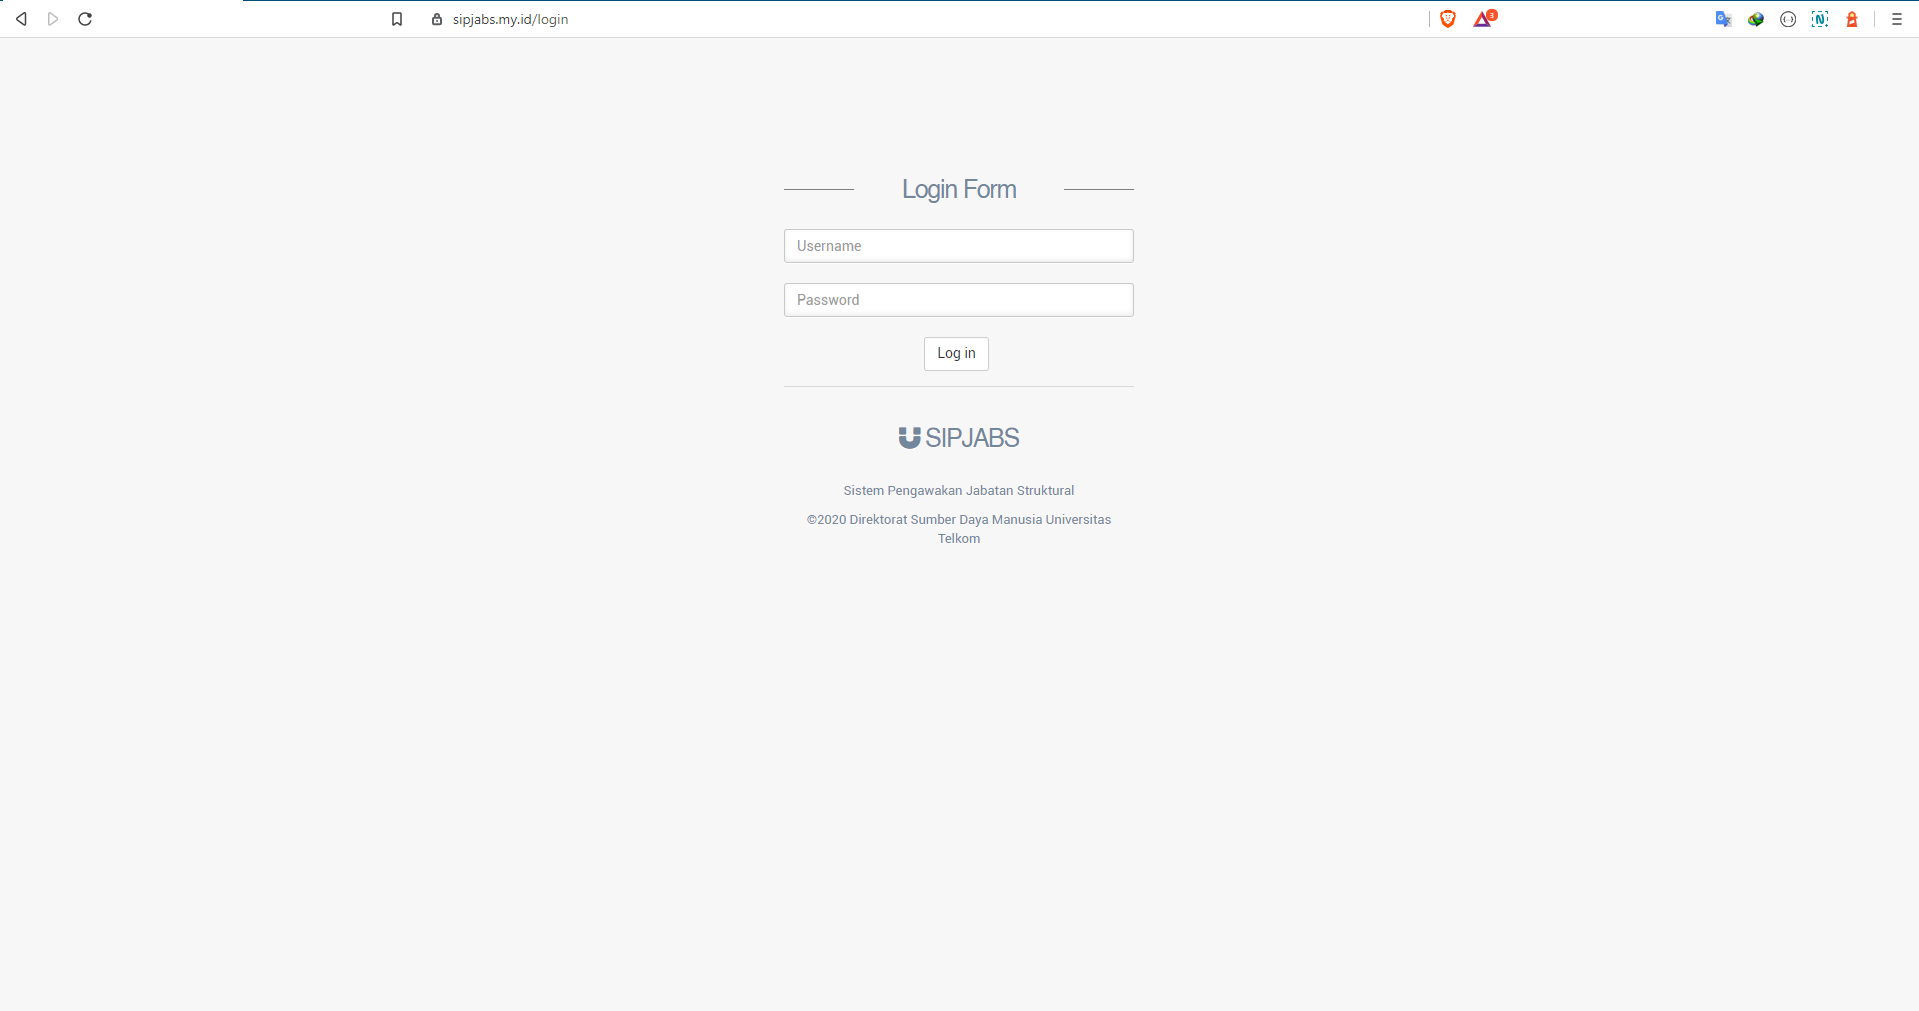
\includegraphics[width=0.65\textwidth, height=60mm]{pics/pengujian/pf1-1.png}}   \\
	
		
		& 2. Inputkan username : zakariawahyu dan password : admin pada form login berikut.
		\raisebox{-\totalheight}{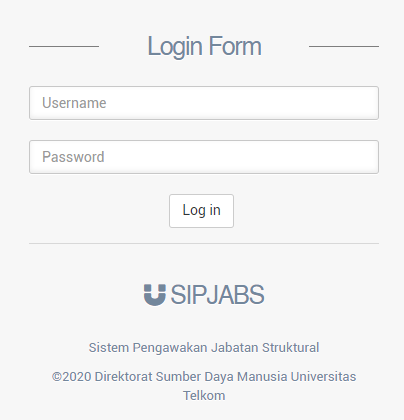
\includegraphics[width=0.4\textwidth, height=60mm]{pics/pengujian/pf1-2.png}}  \\
	
		
		& 3. Klik button ‘Login’ untuk menyelesaikan proses login \\
		\hline
	
		Kriteria Keberhasilan & Sistem akan menampilkan halaman dashboard admin \\
		\hline
		
		Kondisi khusus & Username dan password sudah diberikan oleh admin \\
		\hline
		
		\multirow{2}{*}{Hasil} & Valid : Yes \\
		
		& Invalid : No \\
		\hline
		
		
	\end{tabular}
\end{table}

\begin{table}
	\caption{Tabel Pengujian Login User}
	\centering
	\begin{tabular}{ | l | p{92mm} |}
		\hline
		
		Nomor Test & PF-O2  \\
		\hline
		
		Pengguna & User  \\
		\hline
		
		Judul & Login User  \\
		\hline
		
		\multirow{3}{*}{Teknik} & 
		1. Membuka website dengan mengunjungi link www.sipjabs.my.id dan akan muncul halaman login
		\raisebox{-\totalheight}{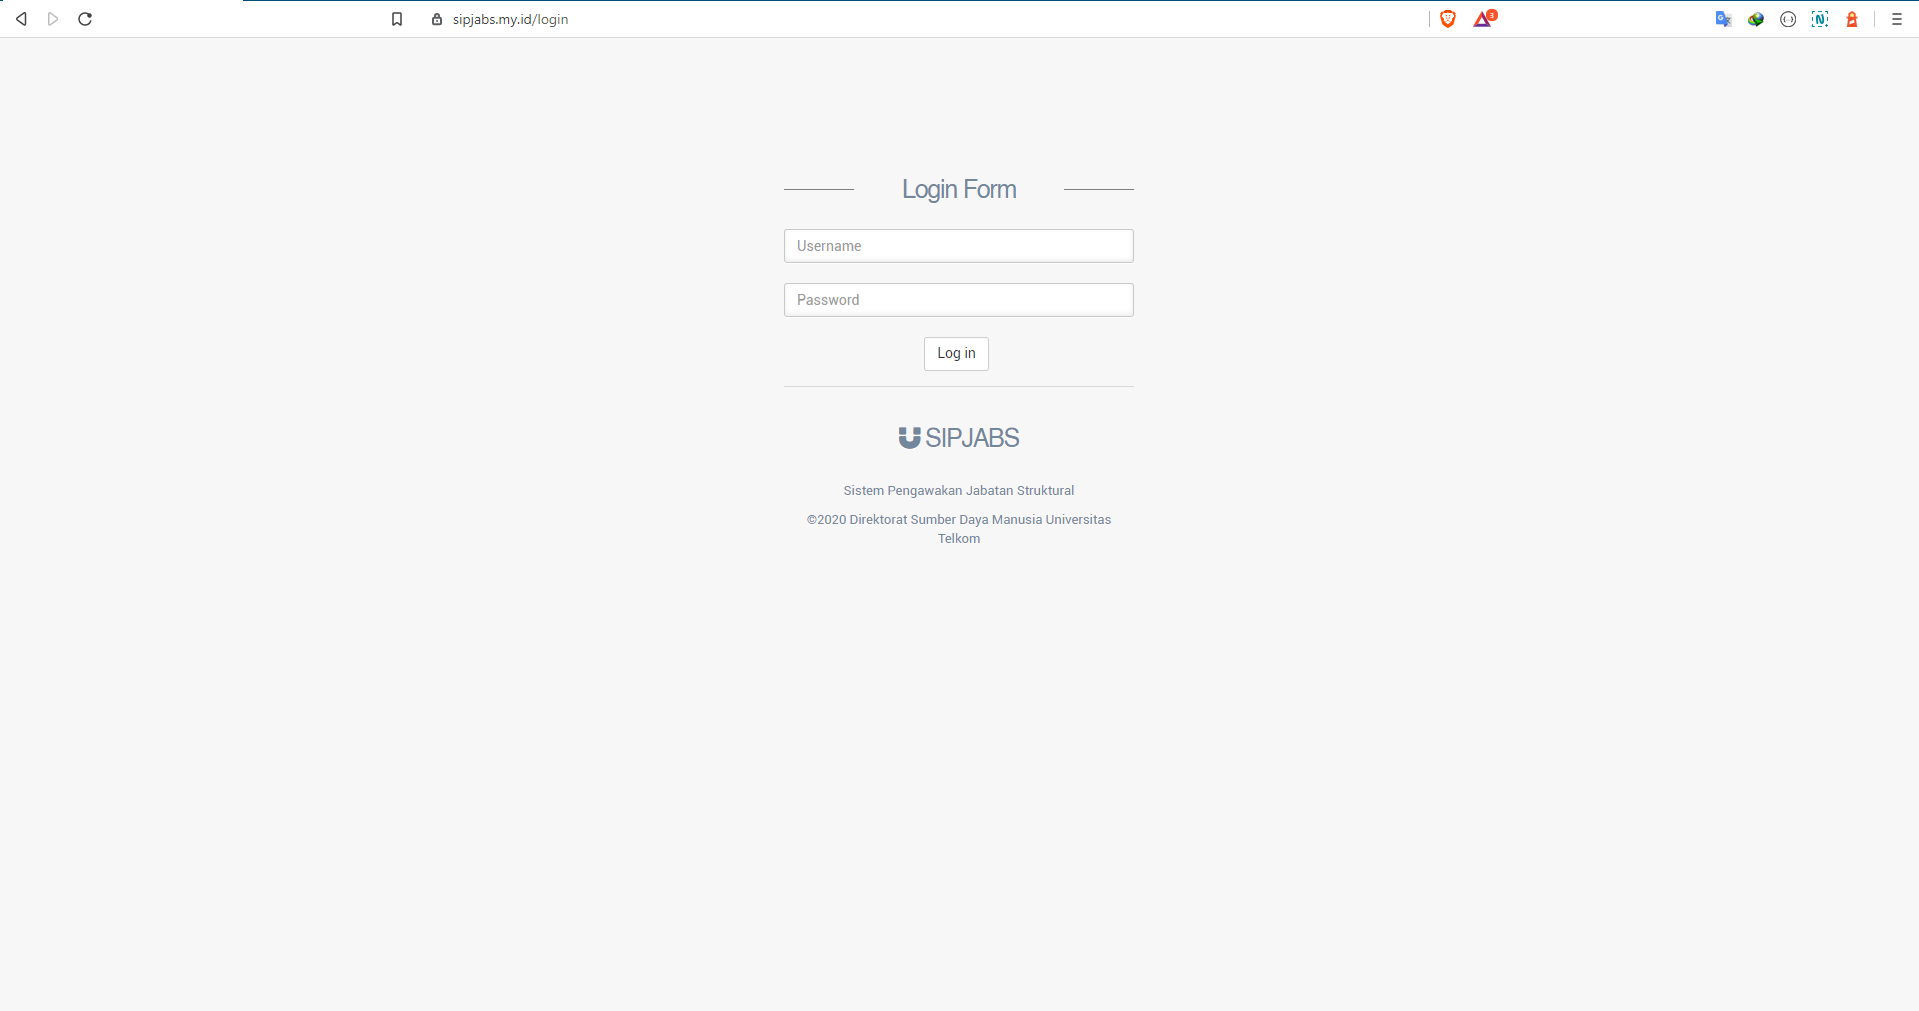
\includegraphics[width=0.65\textwidth, height=60mm]{pics/pengujian/pf1-1.png}}   \\

		
		& 2. Inputkan username : elsajelista dan password : user pada form login berikut.
		\raisebox{-\totalheight}{\includegraphics[width=0.4\textwidth, height=60mm]{pics/pengujian/pf1-2.png}}  \\

		
		& 3. Klik button ‘Login’ untuk menyelesaikan proses login \\
		\hline
		
		Kriteria Keberhasilan & Sistem akan menampilkan halaman dashboard user \\
		\hline
		
		Kondisi khusus & Username dan password sudah diberikan oleh admin \\
		\hline
		
		\multirow{2}{*}{Hasil} & Valid : Yes \\

		
		& Invalid : No \\
		\hline
		
		
	\end{tabular}
\end{table}

\begin{table}
	\caption{Tabel Pengujian Cari Kandidat}
	\centering
	\begin{tabular}{ | l | p{92mm} |}
		\hline
		
		Nomor Test & PF-03  \\
		\hline
		
		Pengguna & User  \\
		\hline
		
		Judul & Cari Kandidat  \\
		\hline
		
		\multirow{3}{*}{Teknik} & 
		1.	Klik “Cari Kandidat” pada menu yang ada di sebelah kiri
		\raisebox{-\totalheight}{\includegraphics[width=0.3\textwidth, height=10mm]{pics/pengujian/pf3-1.png}}   \\
		
		
		& 2. Inputkan persyaratan umum seperti jabatan yang akan di tuju atau posisi target, kemudian dengan minimal jabatan dan kerja minimal.
		\raisebox{-\totalheight}{\includegraphics[width=0.6\textwidth, height=50mm]{pics/pengujian/pf3-2.png}}  \\
		
		
		& 3. Klik button ‘Cari’ untuk melakukan proses pencarian \\
		\hline
		
		Kriteria Keberhasilan & Sistem akan menampilkan nama-nama kandidat \\
		\hline
		
		Kondisi khusus & - \\
		\hline
		
		\multirow{2}{*}{Hasil} & Valid : Yes \\
		
		
		& Invalid : No \\
		\hline
		
		
	\end{tabular}
\end{table}

\begin{table}
	\caption{Tabel Pengujian Filtering}
	\centering
	\begin{tabular}{ | l | p{92mm} |}
		\hline
		
		Nomor Test & PF-04  \\
		\hline
		
		Pengguna & User  \\
		\hline
		
		Judul & Melakukan Filtering  \\
		\hline
		
		\multirow{4}{*}{Teknik} & 
		1.	Klik button “Cari”  untuk memulai mencari kandidat \\
		
		
		& 2. Maka sistem akan menampilkan halaman filter kandidat seperi dibawah ini sesuai persyaratan yang telah di inputkan sebelumnya.
		\raisebox{-\totalheight}{\includegraphics[width=0.5\textwidth, height=40mm]{pics/pengujian/pf4-1.png}}  \\
		
		
		& 3.User dapat memilih persyaratan lebih spesifik untuk menfilter kandidat seperti gambar dibawah ini.
		\raisebox{-\totalheight}{\includegraphics[width=0.4\textwidth, height=40mm]{pics/pengujian/pf4-2.png}} \\

		
		& 4. Lalu sistem akan menampilkan nama-nama kandidat dari hasil filter secara spesifik.
		\raisebox{-\totalheight}{\includegraphics[width=0.5\textwidth, height=40mm]{pics/pengujian/pf4-3.png}}  \\
		\hline
		
		Kriteria Keberhasilan & Sistem akan menampilkan nama-nama kandidat \\
		\hline
		
		Kondisi khusus & - \\
		\hline
		
		\multirow{2}{*}{Hasil} & Valid : Yes \\
		
		
		& Invalid : No \\
		\hline
		
		
	\end{tabular}
\end{table}

\begin{table}
	\caption{Tabel Pengujian Pilih Kandidat}
	\centering
	\begin{tabular}{ | l | p{92mm} |}
		\hline
		
		Nomor Test & PF-05  \\
		\hline
		
		Pengguna & User  \\
		\hline
		
		Judul & Melakukan Pemilihan Kandidat  \\
		\hline
		
		\multirow{3}{*}{Teknik} & 
		1.	Setelah menfilter kandidat, user dapat memilih kandidat untuk dijadikan kandidat sementara. \\
		
		
		& 2.	Sistem akan menampilkan beberapa nama kandidat yang telah terfilter, kemudian user dapat klik button pilih pada salah satu nama kandidat yang akan dipilih.
		
		\raisebox{-\totalheight}{\includegraphics[width=0.5\textwidth, height=40mm]{pics/pengujian/pf5-1.png}}  \\
		
		
		& 3. Data tersebut akan masuk kedalam kandidat sementara 
		\raisebox{-\totalheight}{\includegraphics[width=0.4\textwidth, height=55mm]{pics/pengujian/pf5-2.png}} \\
		\hline
		
		Kriteria Keberhasilan & Sistem akan menampilkan pop-up berhasil ditambahkan kedalam kandidat sementara\\
		\hline
		
		Kondisi khusus & - \\
		\hline
		
		\multirow{2}{*}{Hasil} & Valid : Yes \\
		
		
		& Invalid : No \\
		\hline
		
		
	\end{tabular}
\end{table}

\begin{table}
	\caption{Tabel Pengujian Proses Kandidat}
	\centering
	\begin{tabular}{ | l | p{92mm} |}
		\hline
		
		Nomor Test & PF-06  \\
		\hline
		
		Pengguna & User  \\
		\hline
		
		Judul & Melakukan Pemrosesan Kandidat  \\
		\hline
		
		\multirow{5}{*}{Teknik} & 
		1.	Untuk melanjutkan proses kandidat yang sudah dipilih tadi maka user dapat memprosesnya dengan mengklik icon “Kandidat Sementara” berada pada pojok kanan atas.
		\raisebox{-\totalheight}{\includegraphics[width=0.1\textwidth, height=10mm]{pics/pengujian/pf6-1.png}} \\
		
		
		& 2. Kemudian untuk melihat nama-nama kandidat sementara klik button “View Kandidat  Sementara” 
		
		\raisebox{-\totalheight}{\includegraphics[width=0.5\textwidth, height=10mm]{pics/pengujian/pf6-2.png}}  \\
		
		
		& 3.	Maka sistem akan menampilkan halaman kandidat sementara dengan detail data yang telah ditentukan sebelumnya
		\raisebox{-\totalheight}{\includegraphics[width=0.6\textwidth, height=45mm]{pics/pengujian/pf6-3.png}} \\
		
		& 4.	Kemudian user dapat memilih nama yang akan di proses untuk dijadikan kandidat dengan mengklik button  "Proses kandidat" \\
		
		& 5.	Maka data akan masuk ke dalam data kandidat \\
		\hline
		
		Kriteria Keberhasilan & Sistem akan menampilkan pop-up berhasil memproses kandidat\\
		\hline
		
		Kondisi khusus & - \\
		\hline
		
		\multirow{2}{*}{Hasil} & Valid : Yes \\
		
		
		& Invalid : No \\
		\hline
		
		
	\end{tabular}
\end{table}

\begin{table}
	\caption{Tabel Pengujian Cetak PDF}
	\centering
	\begin{tabular}{ | l | p{92mm} |}
		\hline
		
		Nomor Test & PF-07  \\
		\hline
		
		Pengguna & User  \\
		\hline
		
		Judul & Melakukan Cetak PDF  \\
		\hline
		
		\multirow{4}{*}{Teknik} & 
		1.	Untuk mencetak hasil kandidat maka user harus masuk ke halaman data kandidat dengan cara klik "Data Kandidat" pada menu.
		
		\raisebox{-\totalheight}{\includegraphics[width=0.3\textwidth, height=10mm]{pics/pengujian/pf7-1.png}} \\
		
		
		& 2.	Kemudian sistem akan menampilkan halaman data kandidat dengan nama-nama kandidat yang sudah diproses   
		
		\raisebox{-\totalheight}{\includegraphics[width=0.5\textwidth, height=50mm]{pics/pengujian/pf7-2.png}}  \\
		
		
		& 3.	Lalu user dapat mencetak hasil kandidat dengan klik button "Print PDF"  pada salah satu nama kandidat yang hasilnya akan dicetak. \\
		
		&4.	Sistem akan melakukan proses download laporan kandidat dalam bentuk PDF yang dapat diunduh oleh user   \\
		
		\hline
		
		Kriteria Keberhasilan & Terdapat file pdf yang bisa di unduh\\
		\hline
		
		Kondisi khusus & - \\
		\hline
		
		\multirow{2}{*}{Hasil} & Valid : Yes \\
		
		
		& Invalid : No \\
		\hline
		
		
	\end{tabular}
\end{table}

\newpage
\subsubsection{Pengujian Kesesuaian}

\begin{table}
	\caption{Tabel Pengujian Kesesuaian}
	\centering
	\begin{tabular}{ | l | p{92mm} |}
		\hline
		
		Nomor Test & PK-01  \\
		\hline
		
		Judul & Melakukan pengujian kesesuaian pada aplikasi  \\
		\hline
		
		\multirow{2}{*}{Teknik} & 
		1. Membuka aplikasi pada google chrome \\
		& 2. Membuka aplikasi pada mozila firefox  \\
		\hline
		
		Kriteria Keberhasilan & Menampilkan output yang sama di semua platform browser yang digunakan untuk menguji\\
		\hline
		
		\multirow{3}{*}{Alat Pengujian} & 
		1. Laptop MSI GL62M\\
		& 2. Google Chrome  \\
		& 3. Mozila Firefox \\
		\hline
		
		Kondisi khusus & - \\
		\hline
		
		\multirow{2}{*}{Hasil} & 1. Google Chrome
		
		\raisebox{-\totalheight}{\includegraphics[width=0.65\textwidth, height=20mm]{pics/pengujian/chrome/pk-1.png}}
		
		\raisebox{-\totalheight}{\includegraphics[width=0.65\textwidth, height=20mm]{pics/pengujian/chrome/pk-2.png}}
		
		\raisebox{-\totalheight}{\includegraphics[width=0.65\textwidth, height=20mm]{pics/pengujian/chrome/pk-3.png}}
		\\
		
		
		& 2. Mozila Firefox 
		
		\raisebox{-\totalheight}{\includegraphics[width=0.65\textwidth, height=20mm]{pics/pengujian/firefox/pk-1.png}}
		
		\raisebox{-\totalheight}{\includegraphics[width=0.65\textwidth, height=20mm]{pics/pengujian/firefox/pk-2.png}}
		
		\raisebox{-\totalheight}{\includegraphics[width=0.65\textwidth, height=20mm]{pics/pengujian/firefox/pk-3.png}}\\
		\hline
		
		
	\end{tabular}
\end{table}

%-----------------------------------------------------------------------------%
\subsection{Pengujian Beta}
%-----------------------------------------------------------------------------%
Pengujian beta dilakukan dengan pengujian secara langsung kepada pengguna, salah satu pengujian beta yaitu dengan menggunakan Usability Testing. Berikut hasil pengujiannya:

\begin{table}
	\caption{Tabel Usability Testing}
	\centering
	\begin{tabular}{ | p{5mm} | p{62mm} | c | c | c | c | c | c |}
		\hline	
		
		\multirow{2}{*}{No} & \multirow{2}{*}{Pertanyaan} & \multicolumn{4}{|c|}{Aspek Usability} &  \multirow{2}{*}{Total} & \multirow{2}{*}{Likert} \\
		
		 \cline{3-6} & & STS & TS & S & SS & Skor & \\
		 \hline
		 
		 \multicolumn{8}{|c|}{Aspek Fungsionalitas} \\
		 \hline
		 
		 1 & Apakah semua fitur aplikasi SiPJabS dapat berjalan sesuai dengan fungsinya? &  &  &5 & 3 & 27 & 84,3\% \\
		 \hline
		 
		  2 & Apakah aplikasi SiPJabS mudah untuk digunakan dan dioperasikan? &  &  &4 & 4 & 28 & 87,5\% \\
		 \hline
		 
		 3 & Apakah respon aplikasi SiPJabS baik dan cepat? &  & 1  & 5 & 2 & 23 & 78,1\% \\
		 \hline
		 
		 \multicolumn{7}{|c|}{Rata-rata} & 83,2\% \\ 
		 \hline
		 
		 \multicolumn{8}{|c|}{Aspek Keguaan} \\
		 \hline
		 
		 4 & Apakah aplikasi SiPJabS mudah untuk mencari kandidat secara tepat dan efektif? &  & 1 &6 & 1 & 24 & 75,5\% \\
		 \hline
		 
		 5 & Apakah persyaratan yang diberikan (Filter Pegawai) sudah sesuai dengan job description yang akan dicari? &  & 2 &4 & 2 & 24 & 75,5\% \\
		 \hline
		 
		 6 & Apakah aplikasi SiPJabS sudah layak untuk digunakan pada perusahaan? &  & 2 &4 & 2 & 24 & 75,5\% \\
		 \hline
		 
		  \multicolumn{7}{|c|}{Rata-rata} & 75,5\% \\ 
		 \hline
		 
		 \multicolumn{8}{|c|}{Aspek UI/UX} \\
		 \hline
		 
		 7 & Apakah bentuk button (tombol) pada aplikasi SiPJabS sudah sesuai? &  & 1 &5 & 2 & 25 & 78,1\% \\
		 \hline
		 
		 8 & Apakah warna yang diterapkan pada aplikasi SiPJabS sudah sesuai? &  & 2 &4 & 2 & 24 & 75,5\% \\
		 \hline
		 
		 9 & Apakah icon pada aplikasi SiPJabS sudah sesuai? &  &  &7 & 1 & 8 & 78,1\% \\
		 \hline
		 
		 \multicolumn{7}{|c|}{Rata-rata} & 77,3\% \\ 
		 \hline
		 
	\end{tabular}
\end{table}

Keterangan skor nilai:
\begin{enumerate}
	\item Sangat Tidak Setuju = 1
	\item Tidak Setuju = 2
	\item Setuju = 3
	\item Sangat Setuju = 4
\end{enumerate}

Rumus :	
	$ Hasil akhir = \frac{Total Skor}{Y} x 100 \% $
	
\begin{itemize}
	
	\item Jumlah responden = 8
	\item Y = Jumlah Responden x 4
	
\end{itemize}


%-----------------------------------------------------------------------------%
\section{Diskusi Hasil Pengujian}
%-----------------------------------------------------------------------------%
Pada pengujian aplikasi SiPJabS menggunakan 2 motode yaitu dengan pengujian alpha dan pengujian beta. Untuk pengujuan alpa terdiri dari pengujian fungsionalitas dan pengujian kesesuaian. Hasil dari pengujian fungsionalitas adalah baik dan memandakan fungsionalitas dari SiPJabS dapat berfungsi dengan baik sedangkan untuk hasil pengujian keseuaian adalah baik dengan sesuainya aplikasi ketika dibuka dalam Google Chrome dan Mozila Firefox. 

Untuk pengujian beta menggunakan metode usability testing. Usability testing adalah mencari permasalahan dalam penggunaan aplikasi dan dilakukan dengan membuat sebuah kuesioner untuk menguji seberapa jauh pemahaman pengguna terhadap aplikasi serta menentukan kepuasan pengguna dengan aplikasi sipjabs. Berikut hasil usability testing: 


\begin{enumerate}
	\item Fungsionalitas berjalan dengan baik dengan rata-rata skor likert 83,7\% dengan data tersebut dapat diketahui bahwa pengguna setuju aplikasi SiPJabS memiliki fungsionalitas baik dan dapat digunakan.
	
	\item Apliaksi membantu dalam pencarian kandidat dengan rata-rata skor likert  75,5\% dengan data tersebut dapat disimpulkan aplikasi SiPJabS dapat membantu pengguna dalam pencarian kandidat secara cepat dan efisien. 
	
	\item Aspek desain UI/UX memiliki rata-rata skor likert 77,3 \% dengan data tersebut aspek UI/UX dapat disimpulkan bahwa pengguna setuju desain UI/UX aplikasi SiPJabS baik dan dapat digunakan.
	
	
\end{enumerate} 
